\documentclass[a4paper,11pt]{article}
  \usepackage[T1]{fontenc}
  \usepackage[utf8]{inputenc}
  \usepackage[italian]{babel}
  \usepackage{tabularx}
  \usepackage[font=small,labelfont=bf]{caption}
  \usepackage[footskip=0.4in,margin=2.5cm]{geometry}
  \usepackage{enumitem}
  \usepackage{graphicx}
  \usepackage{amssymb}
  \usepackage{wrapfig}
  \usepackage[dvipsnames]{xcolor}
  \usepackage{listings}
  \usepackage{fancyvrb}
  \usepackage{color}
  \usepackage{mathtools}
  \usepackage{nameref}
  \usepackage{array,collcell}
  \usepackage{float}
  \usepackage{subfig}
  \usepackage{minted} % Needs to be above csquotes.
  \usepackage{csquotes} % Quotes
  \usepackage{booktabs} % For \toprule, \midrule and \bottomrule
  \usepackage{caption}
  \usepackage{longtable}
  \usepackage{amssymb}
  \usepackage{hyperref}

\newminted{c++}{
    frame=leftline,
    framesep=2mm,
    baselinestretch=1.2,
    fontsize=\footnotesize,
    fontfamily=courier,
    escapeinside=@@,
    rulecolor=black
}

  \captionsetup[table]{position=bottom}

  % Setup hyperref
  \hypersetup{
    colorlinks=true,
    linkcolor=NavyBlue,
    filecolor=magenta,
    urlcolor=cyan,
    pdftitle={Algoritmi Avanzati - Laboratorio 2},
    bookmarks=true,
    pdfpagemode=FullScreen,
  }

  % \usepackage{amsmath}
  \DefineShortVerb{\|}
  \fontfamily{arial}

   % C++ code setting

  \newcommand{\tablepath}{tables}

  \makeatletter
  \newcommand{\includetable}[1]{%
    \@ifundefined{tablepath}{%
      \InputIfFileExists{#1}{}{}%
    }{%
      \InputIfFileExists{\tablepath/#1}{}{\InputIfFileExists{#1}{}{}}%
    }
  }
  \makeatother

  \definecolor{diagcolor}{RGB}{146, 151, 192}
  \newcommand\diagid[0]{\textcolor{diagcolor}{$ (\Delta) $}}
  \DeclarePairedDelimiter{\norm}{\lVert}{\rVert}
  \newcommand\norminf[1]{\norm*{#1}_{\infty}}
  \newcommand\detox[1]{\ttfamily\detokenize{#1}}
  \newcommand\strong[1]{\textbf{#1}}

  \newcommand\complexity[1]{$\mathcal{O}(${#1}$)$}
  \newcommand\complexityConstant[0]{\complexity{$1$}}

  \newcommand\complexityNSquared[0]{\complexity{$n^2$}}
  \newcommand\complexityNDegree[0]{\complexity{$degree(n)$}}
  \newcommand\complexityNPlusM[0]{\complexity{$n + m$}}
  \newcommand\complexityM[0]{\complexity{$m$}}
  \newcommand\complexityN[0]{\complexity{$n$}}
  \newcommand\complexityMN[0]{\complexity{$m n$}}
  \newcommand\complexityMLogN[0]{\complexity{$m \cdot log(n)$}}
  \newcommand\complexityLogN[0]{\complexity{$\log_{2}({n})$}}
  \newcommand\complexityLogkN[0]{\complexity{$\log_{k}({n})$}}
  \newcommand\complexityKLogkN[0]{\complexity{$k \cdot \log_{k}({n})$}}
  \newcommand\complexityAlpha[0]{\complexity{$\log_{*}({n})$}}
  \newcommand\complexityMLogM[0]{\complexity{$m \cdot log(m)$}}

  \newcommand\complexityCompleteGraph[0]{$m = $ \complexityNSquared{}}
  \newcommand\complexityHeldKarpTime[0]{\complexity{$2^n \cdot n^2$}}

  \newcommand\bigO[1]{\mathcal{O}(#1)}

  \newcommand\codeinline[1]{\texttt{#1}}  % alternatives: \mintinline{bash}{#1} or \mintinline{c++}{#1} or \textit{#1}

  \begin{document}

    \author{
  Lucchetta Bryan\\
  \texttt{1237584}
  \and
  Parolari Luca\\
  \texttt{1236601}
  \and
  Schiabel Alberto\\
  \texttt{1236598}
}

\title{Algoritmi Avanzati - Laboratorio 2 \\
  \large Travelling Salesman Problem}

\maketitle

\setcounter{tocdepth}{2}
{
  \hypersetup{linkcolor=black}
  \tableofcontents
  \newpage
  \listoffigures
  \listoftables
}
\protect\pagebreak[2]

% \vfill

    \cleardoublepage
    \setlist[itemize]{noitemsep}

    \section{Abstract}
\label{cap:abstract}

Questo secondo homework di laboratorio di Algoritmi Avanzati ha lo scopo di implementare e confrontare algoritmi per risolvere il Traveling Salesman Problem nel caso metrico. \\

\noindent Gli algoritmi implementati sono tre:

\begin{enumerate}
    \item Algoritmo 2-approssimato per Metric-TSP basato sul Minimum Spanning Tree. In questo caso per il calcolo dell'MST abbiamo usato l'algoritmo di Prim;
    \item Algoritmo esatto di Held \& Karp, che usa la programmazione dinamica;
    \item Algoritmo che usa l'euristica costruttiva Closest Insertion per Metric-TSP.
\end{enumerate}

\noindent Abbiamo considerato anche alcune estensioni originali rispetto agli algoritmi visti in classe; esse sono discusse e presentate nella sezione \hyperref[cap:extensions-and-originalities]{Estensioni e originalità}. \\

\noindent Il codice è scritto in C++17 ed è opportunamente commentato per facilitarne la comprensione. Non è stata usata alcuna libreria esterna.

\noindent Le risposte alle 2 domande principali dell'homework sono riportate nella sezione \hyperref[cap:performance-analysis]{Analisi delle performance}.

    \section{IDE e compilatore}
\label{cap:language-choice}

Poiché il nostro sistema operativo di sviluppo è Windows 10, abbiamo usato l'IDE Visual Studio 2019 Community e il suo compilatore \textit{MSVC v142 x64/x86}. \\

\noindent Nell'archivio allegato a questa relazione abbiamo incluso un \textit{Makefile} per permettere la compilazione su altri sistemi operativi usando \textit{g++-9}. Il comando da usare per la compilazione è \mintinline{bash}{make all}. Nel caso la versione di \textit{g++} installata sia la 9.x.y ma l'alias esplicito \textit{g++-9} non esista, è possibile sovrascrivere il compilatore usato con il comando \mintinline{bash}{make CXX=g++ all}.

Altri comandi sono disponibili per eseguire test e benchmark degli algoritmi, oppure per eseguire semplicemente i programmi compilati. Ci si riferisca al file \textit{README.md} incluso al progetto.

    \section{Benchmark}
\label{cap:benchmark-process}

Abbiamo deciso di rendere il processo di misurazione del tempo di esecuzione dei nostri algoritmi esterno al codice dei programmi sviluppati.
Il nostro benchmark tiene quindi conto di tutto, ovvero:

\begin{itemize}
    \item Tempo necessario a leggere il file di input in un container \textit{std::vector} temporaneo;
    \item Tempo per trasformare il container temporaneo in una matrice di adiacenza;
    \item Tempo per eseguire l'algoritmo vero e proprio per la risoluzione di TSP e restituire il risultato;
\end{itemize}

\noindent TODO: PARLARE DEGLI SCRIPT DI MISURAZIONE DEI TEMPI

\noindent Le colonne dei file CSV sopracitati sono le seguenti:

\begin{itemize}
    \item \textbf{ms}: tempo in millisecondi per eseguire il programma su un singolo file di input;
    \item \textbf{output}: risultato del programma, ovvero peso dell'MST del grafo letto in input;
    \item \textbf{n}: numero di nodi del grafo letto;
    \item \textbf{m}: numero di archi del grafo letto;
    \item \textbf{filename}: nome del file di input letto.
\end{itemize}

\noindent Per rendere i risultati del benchmark quanto più stabili e affidabili possibile, abbiamo preso le seguenti precauzioni:

\begin{itemize}
    \item Abbiamo usato sempre lo stesso computer per misurare il tempo di esecuzione dei programmi implementati;
    \item Abbiamo chiuso tutti i programmi in foreground e disabilitato quanti più servizi possibile in background;
    \item Abbiamo disabilitato la connessione Internet del computer scelto;
    \item Abbiamo fatto più misurazioni in tempi differenti. Di tutte le misurazioni effettuate è poi stata scelta la minima per elaborazioni e grafici.
\end{itemize}

\noindent Abbiamo definito lo script Python \textit{benchmark/analysis.py} per automatizzare il processo di confronto degli algoritmi e la creazione di tabelle e grafici inseriti in questa relazione. Esso legge i file CSV generati dallo script di benchmark \textit{benchmark.sh}. \\

\noindent Il computer usato per effettuare i benchmark degli algoritmi ha le seguenti caratteristiche:

\begin{itemize}
    \item \textbf{Sistema Operativo}: Windows 10 Education 64 bit;
    \item \textbf{CPU}: Intel Core i5 6600K 3.50 GHz
    \item \textbf{RAM}: 16 GB;
\end{itemize}

    \section{Struttura del codice}
\label{cap:code-structure}

Il progetto è strutturato in un'unica soluzione Visual Studio\footnote{Una soluzione Visual Studio può essere vista come un macro-progetto che contiene più sotto-moduli.} contenente molteplici progetti, uno per ogni algoritmo implementato. Il codice di ogni progetto è contenuto nella omonima cartella. Di seguito l'elenco dei progetti realizzati.

\begin{itemize}
    \item \textbf{TSP2Approximation TODO: Cambiarlo nella soluzione}
    \item \textbf{HeldKarp}
    \item \textbf{FarthestInsertion}
    \item $(*)$ \textbf{SimulatedAnnleaing}
\end{itemize}

\noindent Abbiamo deciso di scegliere \textbf{Farthest Insertion} tra le euristiche costruttive elencate nell'homework.

\noindent I progetti indicati con $(*)$ sono delle estensioni rispetto agli algoritmi inizialmente richiesti.
\\

\noindent La cartella \textit{Shared} contiene le strutture dati custom e alcune classi e metodi di utilità usati
condivisi tra progetti.

\noindent Abbiamo configurato Visual Studio per importare automaticamente i file di header salvati nella cartella \textit{Shared}
durante la compilazione di ogni sottoprogetto. Analogamente, tale cartella è inclusa nella compilazione del \textit{Makefile}, grazie all'opzione \textit{-I} del compilatore \textit{g++}.


    \section{Scelte implementative}
\label{cap:implementation-choices}

\subsection{Rappresentazione del grafo}
\label{sub:graph-representation}

Gli algoritmi di questo homework operano su grafi pesati completamente connessi e non diretti. Ha quindi senso rappresentare ogni grafo con una Matrice di Adiacenza, dato che i grafi sono completi. In questa relazione useremo in maniera ambivalente i termini \textit{Matrice di Adiacenza} e \textit{Matrice delle Distanze}, poiché i grafi sono pesati.

\noindent I dataset contenenti i grafi di input sono in formato standard \textbf{TSPLIB } e riportano le coordinate 2D dei nodi del grafo in due possibili formati:

\begin{itemize}
    \item \textbf{EUC\_2D}: le coordinate rappresentano la posizione nello spazio euclideo a 2 dimensioni. È dunque richiesto il calcolo della distanza euclidea tra ogni nodo, con il valore arrotondato al numero intero più vicino;
    \item \textbf{GEO}: le coordinate rappresentano la latidudine e la longitudine di ogni punto. Il calcolo della distanza tra due punti in questo caso è più complesso, e richiede una conversione preliminari in radianti. Tale conversione avviene nel costruttore della classe \codeinline{point\_geo}, definita nel file \codeinline{Shared/point.h}.
\end{itemize}

\noindent La formula usata per il calcolo della distanza euclidea è mostrata nel listing \ref{listing:euclidean-distance}, mentre la formula usata per calcolare la distanza geodesica è illustrata nel listing \ref{listing:geodesic-distance}. Si noti che tali distanze seguono i criteri di approssimazione a distanze intere definiti nella specifica dell'homework.

\begin{listing}[!ht]
\begin{minted}{c++}
// Shared/euclidean_distance.h

int euclidean_distance(const point::point_2D& i,
                      const point::point_2D& j) noexcept {
    const auto& [x_i, y_i] = i;
    const auto& [x_j, y_j] = j;

    const double x = x_i - x_j;
    const double y = y_i - y_j;

    // distanza euclidea tra i punti i e j
    const double distance = std::sqrt(std::pow(x, 2) + std::pow(y, 2));

    // arrotonda al valore intero più vicino
    return static_cast<int>(std::round(distance));
}
\end{minted}
\caption{Funzione per il calcolo della distanza Euclidea approssimata tra due punti.}
\label{listing:euclidean-distance}
\end{listing}

\begin{listing}[!ht]
\begin{minted}{c++}
// Shared/geodesic_distance.h

int geodesic_distance(const point::point_geo& i,
                      const point::point_geo& j) noexcept {
    // raggio equatoriale approssimato della terra, in km
    constexpr double RRR = 6378.388;

    const auto& [lat_i, long_i] = i;
    const auto& [lat_j, long_j] = j;

    const double q1 = std::cos(long_i - long_j);
    const double q2 = std::cos(lat_i - lat_j);
    const double q3 = std::cos(lat_i + lat_j);

    // distanza geodesica tra i punti i e j, che sono stati convertiti
    // precedentemente in radianti
    const double distance = RRR *
        std::acos(0.5 * ((1.0 + q1) * q2 - (1.0 - q1) * q3)) + 1.0;

    // ritorna la parte intera della distanza geodesica
    return static_cast<int>(std::trunc(distance));
}
\end{minted}
\caption{Funzione per il calcolo della distanza geodesica approssimata tra due punti.}
\label{listing:geodesic-distance}
\end{listing}

\noindent I risultati del calcolo delle distanze (\textit{EUC\_2D} o \textit{GEO} a seconda del dataset di input) sono inseriti nella posizione corrispondente della Matrice delle Distanze.
Una volta calcolate le distanze, le coordinate originali non sono mantenute: non sono infatti necessarie ai fini della rappresentazione del grafo e del calcolo della soluzione di TSP.
Nella figura \ref{fig:distancematrix-example} è possbile vedere un esempio di una conversione di un grafo di esempio rappresentato da cordinate EUC\_2D nella sua matrice delle distanze. \\

\begin{figure}[h]
	\centering
	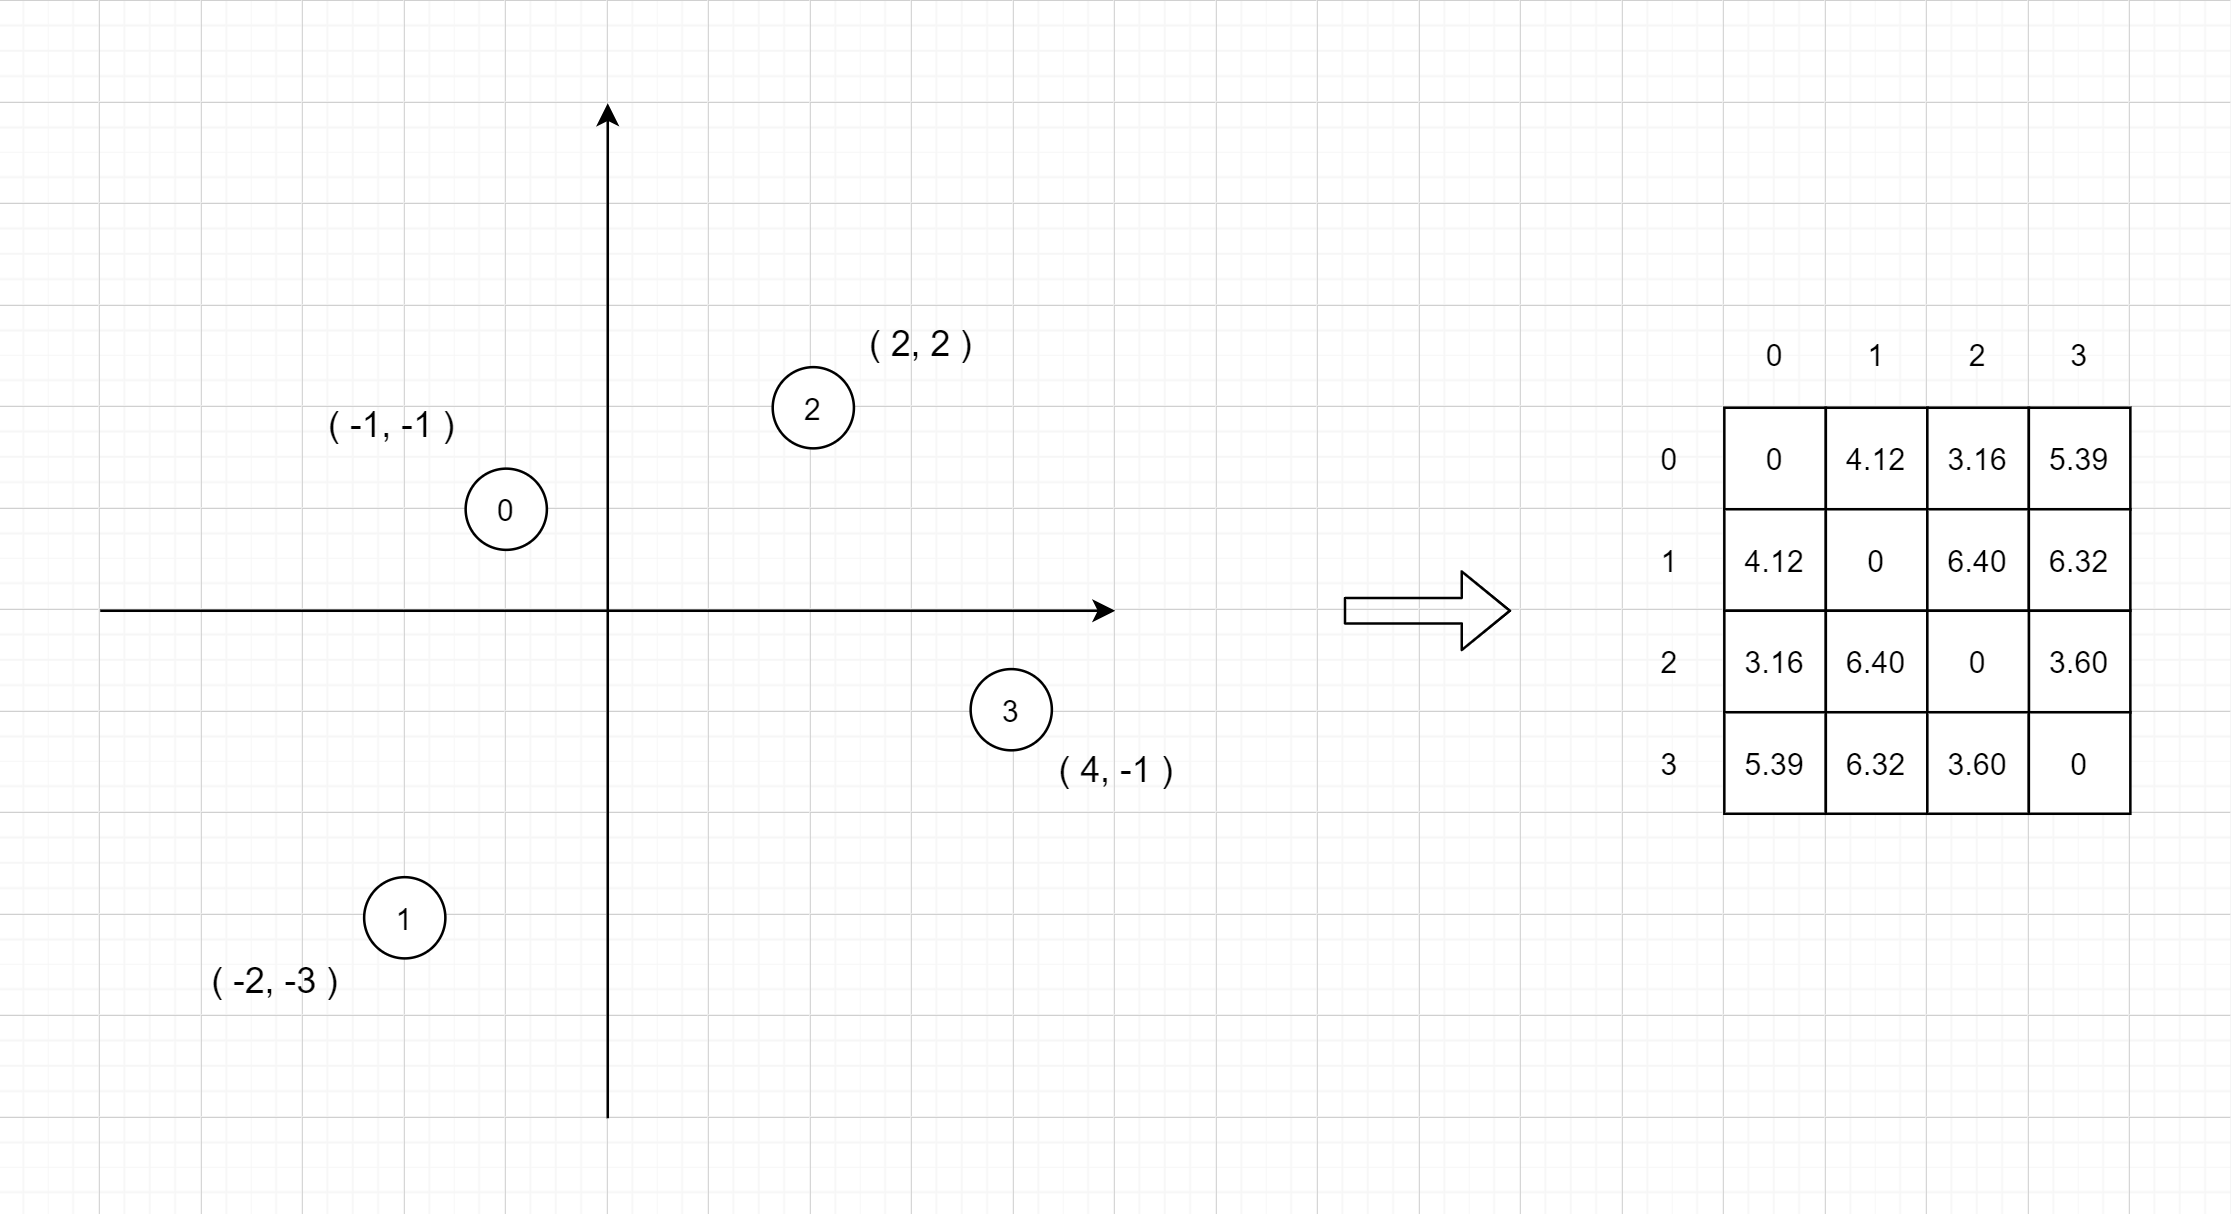
\includegraphics[width=0.9\textwidth]{./images/Distance Matrix.png}
	\caption{Grafo di esempio in uno spazio Euclideo rappresentato con Matrice delle distanze.}
	\label{fig:distancematrix-example}
\end{figure}

\noindent Come nel precedente homework, per semplificare la logica di indicizzazione dei nodi del grafo, la label dei nodi (originariamente numerata da $1$ a $n$) è decrementata di 1, quindi i nodi sono rappresentati dall'intervallo numerico $[0, n-1]$.

\noindent La classe che rappresenta la Matrice delle Distanze dei grafi è definita in \codeinline{DistanceMatrix.h} nella cartella \textit{Shared}.

\begin{listing}[!ht]
\begin{minted}{c++}
std::vector<T> data;

// mappa la coppia di indici (row, column) della matrice in un indice per
// il vettore 1-dimensionale data. (Indicizzazione fisica)
[[nodiscard]] size_t get_index(size_t row, size_t column) const noexcept {
    return row * n_vertexes + column;
}

// valore della distanza tra i nodi (i, j). (Indicizzazione virtuale)
[[nodiscard]] T& at(size_t i, size_t j) noexcept {
    return data.at(get_index(i, j));
}
\end{minted}
\caption{Indicizzazione virtuale e fisica della classe \codeinline{DistanceMatrix.h}.}
\label{listing:virtual-physica-addressing}
\end{listing}

\paragraph{Ottimizzazioni}\mbox{} \\

\noindent Poichè i grafi in esame sono non diretti ($\forall i,j \in V$, $c(i,j) = c(j,i)$), la Matrice delle Distanze è una matrice simmetrica con tutte le entry della diagonale principale pari a 0 (in quanto ogni vertice dista 0 da se stesso).
Abbiamo quindi calcolato le distanze \textit{pair-wise} solo per la parte triangolare superiore della matrice, per poi copiarle in maniera trasposta nella parte triangolare inferiore. Questo ci ha permesso quindi di evitare di calcolare le stesse distanze più volte. \\

\noindent La matrice è rappresentata da un singolo \codeinline{std::vector}. Questo dà la garanzia che ogni riga della matrice sia definita in sezioni contigue di memoria, riduce l'overhead rispetto ad un approccio \codeinline{std::vector<std::vector>}, e, nonostante la logica di indicizzazione sia un po' più complessa (l'indicizzazione virtuale è a due dimensioni, quella fisica è ad una sola dimensione), il cache behaviour della classe è migliore, dando risultati mediamente più performanti. Si veda il listing \ref{listing:virtual-physica-addressing} per osservare la relazione tra indirizzamente fisico e virtuale nella classe \codeinline{DistanceMatrix.h}.

\begin{listing}[!ht]
\begin{minted}{c++}
int main(int argc, char** argv) {
    if (argc != 2) {
        std::cerr << "1 argument required: filename" << std::endl;
        exit(0);
    }

    const char* filename = argv[1];

    // legge il grafo completo non diretto dal file di input
    auto point_reader(read_file(filename));

    // crea la matrice di distanza, usando le distanze euclidea o geodesica a seconda
    // del tipo di input
    DistanceMatrix<int> distance_matrix = point_reader->create_distance_matrix();

    // calcola il peso della soluzione TSP individuata dall'algoritmo
    const auto total_weight = ...;

    // stampa la soluzione trovata
    std::cout << std::fixed << total_weight << std::endl;
}
\end{minted}
\caption{Scheletro comune ad ogni file \codeinline{main.cpp} del progetto.}
\label{listing:main-cpp}
\end{listing}

\subsection{Lettura del Grafo}

\noindent Il file \codeinline{main.cpp} ha la stessa struttura per ogni algoritmo, si veda il listing \ref{listing:main-cpp}. Ad alto livello, le operazioni svolte sono:

\begin{enumerate}
    \item Lettura del file di input: il file di input viene parsato da \codeinline{read\_file.h}, e vengono lette solo le informazioni più importanti, ovvero:

    \begin{itemize}
        \item dimensione del grafo;
        \item tipo di distanza (\textit{EUC\_2D} o \textit{GEO});
        \item coordinate del grafo.
    \end{itemize}

    \noindent Abbiamo usato la libreria di file streaming nativa di C++ (\codeinline{fstream}). Abbiamo rappresentato il tipo di distanza con l'\mintinline{c++}{enum} \codeinline{EdgeWeightType.h}, per la quale abbiamo definito l'operatore di lettura \mintinline{c++}{std::istream& operator>>}.

    \item I punti definiti dopo la riga \codeinline{NODE\_COORD\_SECTION} dei dataset di input sono letti con un'istanza polimorfica di \codeinline{PointReader.h}, che interpreta le coordinate in maniera diversa a seconda del valore assunto dall'enumerazione \codeinline{EdgeWeightType}, ovvero a seconda del tipo di distanza del file. Naturalmente, la sottoclasse \codeinline{EuclideanPointReader.h} usa la distanza Euclidea, mentre \codeinline{GeodesicPointReader.h} usa quella geodesica. Le classi dei punti letti in input sono definiti in \codeinline{point.h} (\codeinline{point\_2D} per le coordinate euclidee, \codeinline{point\_geo} per le coordinate geografiche), e per ognuno di essi è stato definito l'operatore di lettura \mintinline{c++}{std::istream& operator>>} adeguato. Questo ci ha permesso di non avere duplicazione di codice per gestire tipi diversi di punti in input. \\

    \noindent La label dei nodi è decrementata di 1 in questa fase di lettura.

    \item Una volta letti i nodi, viene creata la matrice delle distanze applicando il \textit{Template Method Pattern}, usando la nozione di distanza definita dalle sottoclassi di \codeinline{PointReader.h}. Il metodo concreto \codeinline{distance(i, j)} delle sottoclassi è usato nel costruttore di \codeinline{DistanceMatrix} come \textit{higher-order function}. Si veda il listing \ref{listing:point-reader}.
\end{enumerate}

\noindent Tutti i file citati qui sopra sono nella cartella \textit{Shared} del progetto consegnato e sono corredati di ulteriori commenti esplicativi.

\begin{listing}[!ht]
\begin{minted}{c++}
// Shared/PointReader.h

class PointReader {
protected:
  std::fstream& file;
  size_t dimension;

  // calcola la distanza tra i punti i e j
  virtual int distance(size_t i, size_t j) const = 0;

public:
  PointReader(std::fstream& file, size_t dimension) :
    file(file), dimension(dimension) { }

  // distruttore virtual poiché PointReader è una classe base
  virtual ~PointReader() = default;

  // consuma la lista di coordinate dal file di input
  virtual void read() = 0;

  // crea la matrice delle distanze a partire dai punti letti. Usa il metodo distance
  // implementato dalle sotto classi come funzione higher-order
  DistanceMatrix<int> create_distance_matrix() {
    using namespace std::placeholders;
    auto distance_fun(std::bind(&PointReader::distance, this, _1, _2));

    return DistanceMatrix<int>(dimension, distance_fun);
  }
};
\end{minted}
\caption{Definizione parziale di \codeinline{Shared/PointReader.h} che evidenza la creazione della matrice delle distanze del grafo letto.}
\label{listing:point-reader}
\end{listing}

%\subsection{Strutture Dati comuni}

%Tutte le strutture dati elencate di seguito sono definite nella cartella \textit{Shared}.
%Ove possibile, per la nomenclatura dei metodi abbiamo cercato di seguire lo stesso standard dei container STL di C++.
%Inoltre, le strutture dati usate sono sempre pre-allocate in memoria quando possibile, evitando rehashing e riallocazioni dispendiose. Questo significa che la maggior parte delle operazioni indicate con \complexityConstant{} ammortizzato siano in realtà totalmente costanti nella pratica. \\

\subsection{Rappresentazione alternativa del grafo: caso MST}
\label{alternative-graph-representation}

\noindent L'algoritmo di $2$-approssimazione basato sul calcolo del Minimum Spanning Tree fa uso di due rappresentazioni diverse per i grafi.
\codeinline{DistanceMatrix.h} è usato per leggere il grafo in input ed eseguirne l'algoritmo di Prim (che è stato adattato dal precedente homework). \codeinline{AdjacencyMapGraph.h}, che contiene un subset definite per la Mappa di Adiacenza definita nel precedente homework, è invece usata per rappresentare il Minimum Spanning Tree all'interno di \codeinline{DFS.h}, che lo scorre per generare il vettore della visita \textit{pre-order}. Questa scelta è dovuta al fatto che l'MST non è denso come il grafo di input, e anzi contiene solo $n - 1$ archi. Una rappresentazione matriciale è quindi inutilmente costosa in termini di spazio in questo caso.

\newpage
\subsection{Rappresentazione dei circuiti parziali di Held \& Karp}

L'algoritmo Held-Karp richiede esplicitamente l'uso di due vettori:
\begin{itemize}
    \item $d[v,S]$ è il peso del cammino minimo che parte dal nodo $0$ e termina in $v$, visitando tutti i nodi nell'insieme $S$;
    \item $\pi[v,S]$ è il predecessore di $v$ nel cammino minimo definito come sopra.
\end{itemize}

\noindent Poiché l'homework richiede la restituizione del peso del cammino Hamiltoniano inferiore e non il cammino stesso, abbiamo omesso il vettore $\pi[v,S]$. \\

\noindent Abbiamo rappresentato la tabella $d[v,S]$ usata dall'algoritmo di programmazione dinamica come una mappa chiave-valore, dove:

\begin{itemize}
    \item la chiave è una coppia $(S, v)$;
    \item il valore è il peso del cammino minimo che parte dal nodo 0 e termina in $v$, visitando tutti i nodi in $S$.
\end{itemize}

\noindent In \codeinline{C++}, il tipo per rappresentare la mappa corrispondente a $d[v,S]$ è:

\begin{center}
    \mintinline{c++}{std::unordered_map<std::pair<decltype(S), size_t>, int>}
\end{center}

\noindent Poiché le distanze euclidea e geodesica sono approssimate a valori interi, il tipo del valore della mappa è \mintinline{c++}{int}.
Per rappresentare il set di nodi $S$ abbiamo studiato 3 possibili soluzioni.

\subsubsection{Rappresentazione del circuito parziale S}
\label{held-karp-S-repr}

Di seguito sono presentate le 3 possibili soluzioni che abbiamo individuato per rappresentare il circuito parziale $S$ dell'algoritmo di Held \& Karp. Ricordiamo che $S$ fa parte della chiave di una \mintinline{c++}{std::unordered_map}, quindi deve esistere un metodo che definisca l'hash di $S$.

\paragraph{Unordered Set}\mbox{}\\

\noindent La soluzione più semplice per rappresentare un insieme di vertici senza ripetizioni è usare la struttura dati \mintinline{c++}{std::unordered_set}. La tabella \ref{tab:pro-cons-unordered-set} evidenzia i pro e i contro di questo approccio. Osserviamo in particolare che lo spazio occupato per rappresentare un circuito parziale può essere compattato, il che può essere d'aiuto a limitare la RAM occupata, visto che Held \& Karp ha un'occupazione spaziale esponenziale sulla taglia dell'input. \\

\noindent Notiamo inoltre che la libreria standard non definisce alcun metodo \\ \mintinline{c++}{std::hash<std::unordered_set<T>>}, quindi è spettata a noi la definizione della \textit{hash function} per questa struttura dati. Si veda la sezione \ref{hashing} per ulteriori informazioni.

\begin{table}[h]
  \centering
    \begin{tabular}{|c | c|}
    \hline
    \textbf{PRO} & \textbf{CONTRO} \\ [0.5ex]
    \hline\hline
    Offerta dalla libreria standard di C++ & Ha un'occupazione spaziale lineare\\
    \hline
    Rende evidente la non esistenza di nodi ripetuti & La libreria standard non ne definisce l'hash \\
    \hline
    Facile da usare &  \\
    \hline
  \end{tabular}
    \caption{Analisi dei pro e contro di std::unordered\_set.}
    \label{tab:pro-cons-unordered-set}
\end{table}

\noindent Il tipo della mappa che rappresenta $d[v,S]$ in questo caso è:

\begin{center}
    \mintinline{c++}{std::unordered_map<std::pair<std::unordered_set<size_t>, size_t>, int>}
\end{center}

\paragraph{Tecnica bit masking}\mbox{}\\

\noindent \textbf{Premessa}: per questo metodo, abbiamo assunto che i programmi saranno eseguiti solo su architetture a 64 bit. I grafi con più di 63 nodi non possono essere rappresentati con questo metodo. \\

\noindent Una soluzione migliore per rappresentare in maniera estremamente compatta il set di nodi visitati $S$ è usare un singolo numero intero senza segno a 64 bit. In questo caso, ogni bit a 1 rappresenta la presenza di un vertice $i$ nell'insieme $S$.
Se il bit all'$i$-esima posizione nel numero vale 1, allora il vertice $i \in S$, se il bit vale invece 0 allora $i \notin S$. La tabella \ref{tab:pro-cons-bit-masking} evidenzia i pro e i contro di questo approccio. \\

\noindent Nel nostro linguaggio, il tipo necessario a definire numeri interi senza segno a 64 bit è \\
\mintinline{c++}{unsigned long long}. Si consideri l'esempio in figura \ref{fig:bitmasking-example} per vedere come è possibile rappresentare $S$ in questo modo.

\begin{table}[h]
  \centering
    \begin{tabular}{|c | c|}
    \hline
    \textbf{PRO} & \textbf{CONTRO} \\ [0.5ex]
    \hline\hline
    Massima compattezza spaziale & Complesso da usare \\
    \hline
    Rende evidente la non esistenza di nodi ripetuti & Supporta solo architetture a 64 bit \\
    \hline
    La libreria standard ne definisce l'hash & Usabile solo per grafi con $n \leq 63$ \\
    \hline
  \end{tabular}
    \caption{Analisi dei pro e contro della tecnica bit masking per numeri interi senza segno.}
    \label{tab:pro-cons-bit-masking}
\end{table}

\begin{figure}[h]
	\centering
	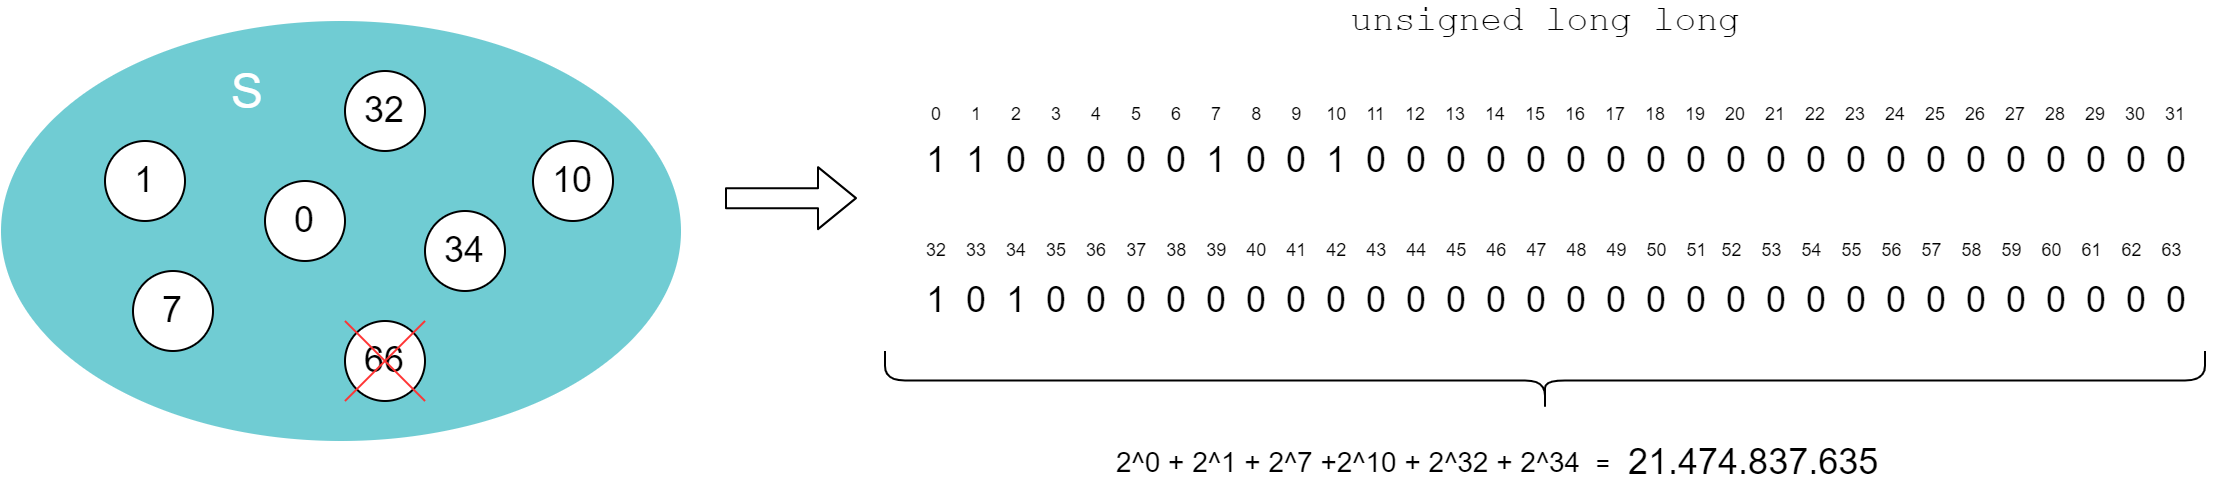
\includegraphics[width=0.9\textwidth]{./images/BitMasking Example.png}
	\caption{Rappresentazione di S tramite BitMasking}
	\label{fig:bitmasking-example}
\end{figure}

\noindent Con questa rappresentazione chiamata \textit{bit masking}, eliminazione, aggiunta e verifica della presenza di vertici in $S$ sono implementate sfruttando operazioni \codeinline{AND}, \codeinline{OR}, \codeinline{XOR}, bit-a-bit e bit-shifting (\mintinline{c++}{<<}). \\

\noindent Poiché questo tipo di operazioni si traduce in una singola istruzione Assembly, manipolare l'insieme $S$ tramite bit-masking è estremamente performante sia dal punto di vista temporale che spaziale. \\

\noindent Un limite di tale struttura è l'impossibilità di poter rappresentare un set $S$ che contiene più di 64 nodi, come è possibile vedere nell'esempio della figura \ref{fig:bitmasking-example} dove il vertice 66 non può essere rappresentato in questo modo. Il limite di rappresentazione di $S$ in realtà scende a 63 nodi per via delle operazioni di bit-shift necessarie a manipolare il circuito parziale.

\noindent Il tipo della mappa in questo caso è:

\begin{center}
    \mintinline{c++}{std::unordered_map<std::pair<unsigned long long, size_t>, int>}
\end{center}

\paragraph{Struttura dati ad-hoc: DynamicBitMasking}\mbox{} \\

\noindent Per superare il limite della rappresentazione tramite BitMasking per più di 63 nodi si è pensato di estendere l'idea del BitMasking non più ad un solo numero, ma a più numeri. In questo modo se l'insieme $S$ può raggiungere dimensioni più grandi di 64 nodi è possibile rappresentarlo con più di un numero, dove il primo numero rappresenta i primi 64 nodi, il secondo i successivi 64 nodi e così via. \\

\noindent Abbiamo dunque creato un'apposita classe definita in \codeinline{HeldKarp/DynamicBitMasking.h} che,  tramite un \mintinline{c++}{std::vector<unsigned long long>}, rappresenta un insieme $S$ di qualunque dimensione. In questo modo, data una posizione di un bit $i$, è sufficiente ricavarsi l'indice del vettore dove risiede il numero che contiene il bit $i$ (tramite la divisione intera di $i$ con 64) e la posizione del bit all'interno del numero (tramite il resto della divisione di $i$ con 64). Nell'esempio raffigurato in figura \ref{fig:DynamicBitMasking-example} è possibile vedere come lo stesso set S visto nell'esempio precedente ora possa essere rappresentato tramite questa nuova struttura dati. \\

\begin{figure}[h]
	\centering
	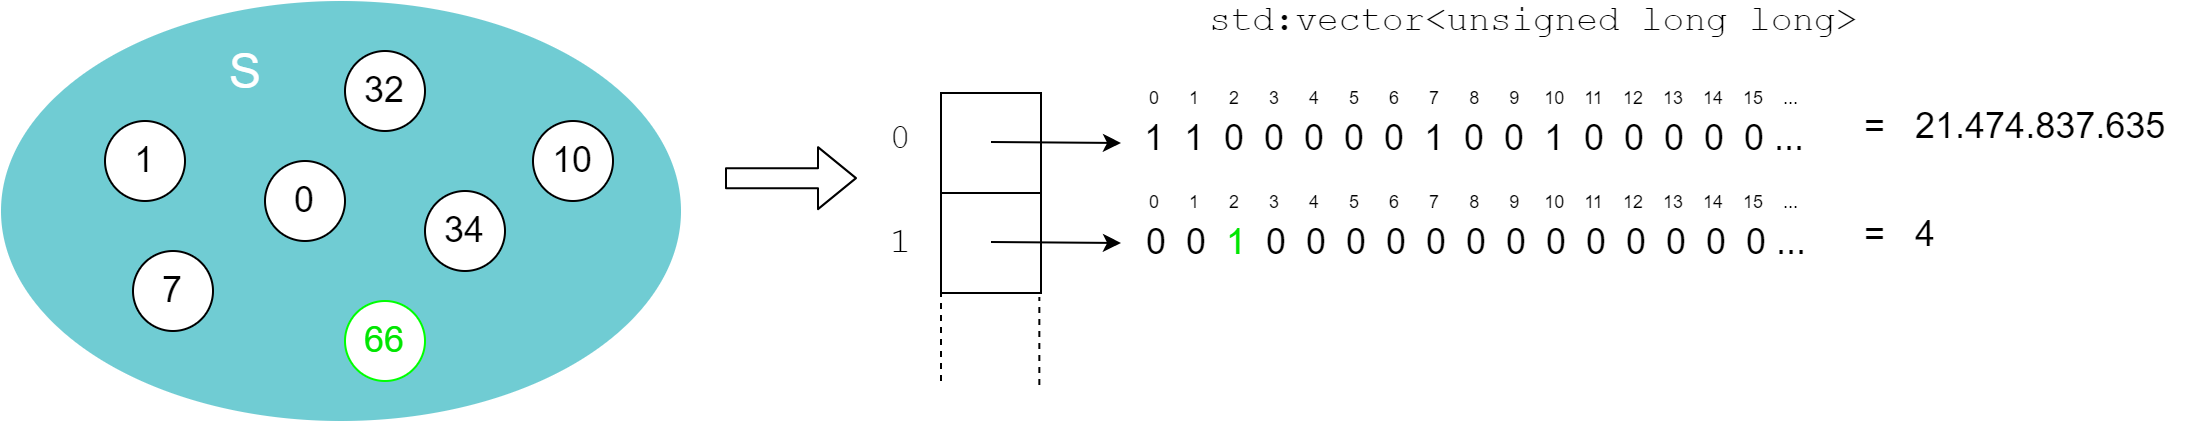
\includegraphics[width=0.9\textwidth]{./images/BitMaskingExtended Example.png}
	\caption{Rappresentazione di S tramite DynamicBitMasking}
	\label{fig:DynamicBitMasking-example}
\end{figure}

\noindent Il tipo della mappa in questo caso è:

\begin{center}
    \mintinline{c++}{std::unordered_map<std::pair<DynamicBitMasking, size_t>, int>}
\end{center}

\subsubsection{Confronto tra std::unordered\_set, bit masking e DynamicBitMasking}

In questa sezione mostriamo un confronto tra le performance in termini di complessità spaziali e temporali delle 3 soluzioni proposte. Nel grafico riportato in figura \ref{fig:UnorderedvsDynamicBitMasking} abbiamo comparato i tempi d'esecuzione di HeldKarp (senza timeout) con le 3 strutture dati descritte nella sezione \ref{held-karp-S-repr}.
Come input, abbiamo considerato i dataset \codeinline{burma14}, \codeinline{ulysses16} e \codeinline{ulysses22}, aventi rispettivamente 14, 16, e 22 nodi.

\begin{figure}[h]
	\centering
	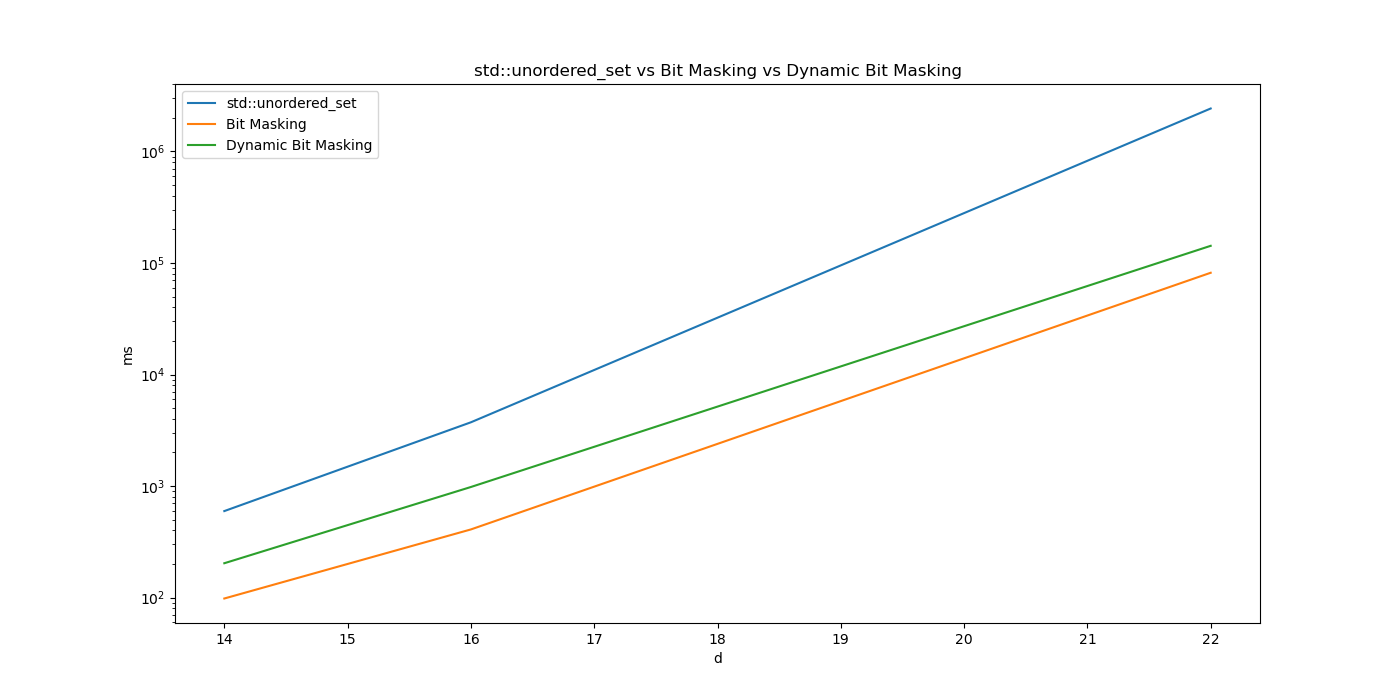
\includegraphics[width=1\textwidth]{./images/unorderedSet vs BitMasking.png}
	\caption{Confronto dei tempi di esecuzione di Held-Karp al crescere del numero di nodi usando unordered\_set, BitMasking ed DynamicBitMasking. I dataset usati per il confronto sono \codeinline{burma14}, \codeinline{ulysses16} e \codeinline{ulysses22}. Si noti che l'asse delle ordinate è in scala logaritmica.}
	\label{fig:UnorderedvsDynamicBitMasking}
\end{figure}

\noindent Com'era prevedibile, l'implementazione più veloce risulta essere l'applicazione della tecnica \textit{bit masking} che manipola un singolo numero intero senza segno a 64 bit; l'overhead delle operazioni in questo caso è infatti minimo, come minima è l'occupazione spaziale ($S$ ha un'uccupazione costante di 8 byte). \\

\noindent \mintinline{c++}{std::unordered_set<size_t>}, al contrario, ha i tempi più esecuzioni più elevati, almeno un ordine di grandezza più lunghi rispetto alla struttura dati realizzata ad-hoc, DynamicBitMasking. \\

\noindent Visti i risultati sperimentali, abbiamo quindi deciso di usare bit-masking a 64 bit per implementare l'algoritmo di Held \& Karp con grafi aventi meno di 64 nodi, e DynamicBitMasking per eseguire Held \& Karp su grafi di dimensioni maggiori.

\subsection{Timeout per Held \& Karp}

\noindent L'algoritmo di Held-Karp ha complessità temporale \complexityHeldKarpTime{}, quindi i tempi di esecuzione \textit{esplodono} anche solo per grafi con poche decine di nodi. Come richiesto dall'homework, all'algoritmo di Held-Karp è assegnato un timeout di esecuzione $T$. Abbiamo fissato il valore di $T$ a 2 minuti, per mantenere la RAM occupata sotto controllo (anche la complessità spaziale dell'algoritmo è esponenziale).\\

\noindent La nostra implementazione di Held-Karp, quindi:

\begin{enumerate}
    \item Ritorna la soluzione esatta se i suoi tempi di esecuzione sono inferiori a 2 minuti, senza aspettare lo scadere del timeout;
    \item Se invece il timeout scade, termina preventivamente la ricorsione e ritorna la migliore soluzione trovata fino a quel momento. A seconda della profondità del call-stack ricorsivo, la soluzione potrebbe essere ritornata qualche secondo dopo lo scadere del timeout.
\end{enumerate}

\noindent C++17 non fornisce soluzione \textit{out-of-the-box} ad alto livello per eseguire funzioni con un limite di tempo. Abbiamo quindi implementato un meccanismo di questo tipo in \codeinline{Shared/timeout.h}, il cui funzionamento ad alto livello è il seguente:

\begin{itemize}
    \item Il thread principale crea un \textit{worker thread} incaricandolo di eseguire Held-Karp sul grafo letto in input. Fa quindi partire il timeout e resta in attesa del risultato del worker thread. Tale risultato sarà disponibile da un \codeinline{std::future}.
    \item Se il worker thread termina prima dello scadere del timeout, il thread principale è immediatamente sbloccato e il risultato della funzione (restituito da \codeinline{std::future::get()}) è ritornato al chiamante.
    \item Se il timeout scade e il worker thread non ha ancora terminato l'esecuzione, il thread principale gli notifica di terminare l'esecuzione il prima possibile. Tale notifica avviene forzando la conclusione di una \codeinline{std::promise} creata dal main thread e data in input alla funzione eseguita incapsulata nella classe \codeinline{timeout\_signal}.
    \item Quando la funzione eseguita si accorge che il tempo a disposizione è scaduto, interrompe la ricorsione e ritorna al chiamante la migliore soluzione individuata fino a quel momento.
\end{itemize}


    \newpage
    
\section{Algoritmi}
\label{cap:algorithms}

\subsection{MST2Approximation}

MST2Approximation è l'implementazione dell'algoritmo di $2$-approssimazione basato sul Minimum Spanning Tree visto a lezione. L'algoritmo prevede i seguenti step:

\begin{enumerate}
    \item Selezionare un vertice radice $root$ arbitrario;
    \item Ricavare l'MST del grafo in input a partire da $root$, utilizzando ad esempio l'algoritmo di Prim;
    \item Eseguire una visita pre-order dell'MST ricavato al passo precedente;
    \item Aggiungere la radice $root$ pre-order alla fine della lista ritornata dalla visita pre-order.
    \item Calcolare il peso totale del circuito ricavato nei 2 passi precedenti e restituire il risultato.
\end{enumerate}

\noindent Il listato \ref{listing:tsp2approx} contiene la nostra implementazione dell'algoritmo, step per step.\\

\begin{listing}[!ht]
\begin{minted}{c++}
// MST2Approximation/approx_tsp.h

// Step 1
random_generator::IntegerRandomGenerator random(0, distance_matrix.size() - 1);
const size_t root = random();

// Step 2
std::vector<Edge> mst(mst::prim_binary_heap_mst(distance_matrix, root));

// Step 3, 4
DFS dfs(std::move(mst));
const auto circuit = dfs.preorder_traversal();

// Funzione lambda che calcola la distanza tra due vertici
const auto get_distance = [&distance_matrix](const size_t x, const size_t y) {
    return distance_matrix.at(x, y);
};

// Step 5
return utils::sum_weights_in_circuit(circuit.cbegin(), circuit.cend(), get_distance);
\end{minted}
\caption{Implementazione di TSP 2-approssimato. I commenti del file originale sono stati omessi per una maggiore compattezza.}
\label{listing:tsp2approx}
\end{listing}

\noindent L'algoritmo TSP 2-approssimato è stato implementato a partire dallo pseudo codice visto in classe. \\

\subsubsection{Osservazioni}

\begin{itemize}
    \item Abbiamo usato l'algoritmo di Prim per eseguire il calcolo del Minimum Spanning Tree. Esso è infatti più adatto rispetto a Kruskal quando il grafo è rappresentato come Matrice della Distanze. Kruskal richiede di estrarre la lista di lati ordinata in modo ascendente rispetto al peso all'inizio dell'algoritmo, mentre Prim necessita solo della lista dei vertici. Ricordiamo che in un grafo completo vale l'equivalenza \complexityCompleteGraph{}.

    \item La coda di priorità usata dall'algoritmo di Prim è stata implementata con una Min Heap binaria, la quale è già stata descritta in dettaglio nella relazione del primo progetto.

    \item Come notato nella sezione \hyperref[alternative-graph-representation]{Rappresentazione alternativa del grafo: caso MST}, l'albero di copertura minimo è rappresentato come Mappa di Adiacenza all'interno di \codeinline{Shared/DFS.h}.

    \item Il metodo \mintinline{c++}{DFS::preorder_traversal} invoca al suo interno il metodo ricorsivo \\
    \mintinline{c++}{DFS::preorder_traversal_rec}. Il listato \ref{listing:dfs} contiene la definizione di tale metodo.
\end{itemize}

\begin{listing}[!ht]
\begin{minted}{c++}
// Shared/DFS.h

void preorder_traversal_rec(size_t v, std::unordered_set<size_t>& visited,
                            std::vector<size_t>& circuit) const {
  visited.insert(v);
  circuit.push_back(v);

  for (const auto& [u, _] : adjacency_map.adjacent_vertexes(v)) {
    // se un nodo adiacente non è stato visitato, viene visitato
    // ricorsivamente
    if (!visited.count(u)) {
      preorder_traversal_rec(u, visited, circuit);
    }
  }
}
\end{minted}
\caption{Implementazione ricorsiva della visita pre-order, inizialmente invocata sul nodo $0$. I commenti del file originale sono stati omessi per una maggiore compattezza.}
\label{listing:dfs}
\end{listing}

\subsection{HeldKarp}

Riportiamo lo pseudocodice dell'algortimo di programmazione dinamica Held \& Karp. La funzione \codeinline{HeldKarp(S, v)} vista a lezione funziona nel seguente modo:

\begin{enumerate}
    \item Caso base 1: verifica se il percorso parziale $S$ contenga un solo nodo, e in caso positivo restituisce la distanza tra il nodo $v$ e il nodo di partenza $0$.
    \item Caso base 2: controlla se la distanza tra i nodi $0$ e $v$, passando per tutti i nodi in $S$, sia già stata calcolata, e in caso positivo restituisce tale valore.
    \item Caso ricorsivo:
    \begin{enumerate}
        \item Step a: Inizializza la distanza minima a $\infty$ e considera $S \setminus {v}$.
        \item Step b: Scansiona tutti i nodi in $S \setminus {v}$, calcolando ricorsivamente la distanza. Se la distanza trovata è inferiore a quelle precedentemente ricavate, viene sostituita.
        \item Step c: Verifica se il timeout è scaduto. In caso positivo, effettua l'unrolling prematuro dello stack di ricorsione e ritorna il miglior risultato ottenuto fino a questo punto.
    \end{enumerate}
    \item Step d: Ritorna la distanza minima calcolata del circuito parziale $S$.
\end{enumerate}

\noindent La nostra implementazione usa due diverse strutture dati per rappresentare il sottoinsieme $S$ tra quelle viste in \ref{held-karp-S-repr}:

\begin{itemize}
    \item \mintinline{c++}{unsigned long long} manipolati tramite bit masking se il grafo in input ha meno di 64 nodi;
    \item \mintinline{c++}{DynamicBitMask} altrimenti.
\end{itemize}

\noindent Il listato \ref{listing:held-karp} contiene la nostra implementazione dell'algoritmo, step per step.

\begin{listing}[!ht]
\begin{minted}{c++}
// HeldKarp/HeldKarp.h
using ull = unsigned long long;
using held_karp_dp_bits_t = std::unordered_map<std::pair<ull, size_t>, int>;

int held_karp_tsp_rec_bits_helper(timeout::timeout_signal& signal,
                                  DistanceMatrix<int>& distance_matrix,
                                  held_karp_dp_bits_t& C,
                                  ull bits, size_t v = 0) {
    // Caso base 1
    if (utils::is_singleton(bits, v)) {
        return distance_matrix.at(v, 0);
    }

    // Case base 2
    if (C.count({bits, v})) {
        return C[{bits, v}];
    }

    // Step a
    int min_dist = std::numeric_limits<int>::max();
    const ull difference = utils::reset_bit(bits, v);
    const size_t n = distance_matrix.size();

    // Step b
    utils::for_each(difference, n, [&](const size_t bit) {
        int dist = held_karp_tsp_rec_bits_helper(signal, distance_matrix, C,
                                                 difference, bit);
        int tmp_dist = dist + distance_matrix.at(v, bit);

        if (tmp_dist < min_dist) {
            min_dist = tmp_dist;
        }

        // Step c
        return !signal.is_expired();
    });

    // Step d
    C[{bits, v}] = min_dist;
    return min_dist;
}

\end{minted}
\caption{Implementazione di Held e Karp con BitMasking. I commenti del file originale sono stati omessi per una maggiore compattezza.}
\label{listing:held-karp}
\end{listing}

\subsubsection{Osservazioni}

\begin{itemize}
    \item Abbiamo voluto riportare qui la versione con BitMasking a 64 bit, la versione con DynamicBitMasking è simile. Il controllo su quale delle due implementazioni usare è fatto prima di lanciare la funzione di ricorsione appropriata.\\
\end{itemize}

\newpage

\subsection{Closest Insertion}
\label{sec:closest-insertion}

Closest Insertion è un'euristica costruttiva per Metric-TSP che
consente di approssimare la soluzione ottima ad un fattore
$\log(n)$. La complessità asintotica di quest'euristica è
$\bigO{n^2}$.

\subsubsection{Idea}

L'euristica è molto semplice e utilizza un'insieme di regole per
scegliere il punto di partenza, il vertice da inserire ad ogni
iterazione e la posizione in cui inserire il nuovo vertice. In
particolare:

\begin{enumerate}
    \item per l'inizializzazione, si considera il circuito parziale composto
      dal solo vertice $0$; si trova un vertice $j$ che minimizza $w(0,
      j)$ e si costruisce il circuito parziale $(0, j,0)$;
    \item per la selezione, si trova un vertice $k$ non presente nel circuito
      parziale $C$ che minimizza $\delta(k,C)$;
    \label{pseudo:closest-insertion-selection}
    \item per l'inserimento, si trova l’arco ${i, j}$ del circuito parziale che
      minimizza il valore $w(i, k) + w(k, j) - w(i, j)$ e lo si inserisce
      $k$ tra $i$ e $j$;
    \item si ripete da \ref{pseudo:closest-insertion-selection} finché
tutti i vertici non sono stati inseriti nel circuito.
\end{enumerate}

\subsubsection{Implementazione}

\noindent Il listato \ref{listing:closest-insertion} contiene la
nostra implementazione dell'algoritmo.

\begin{listing}[!ht]
\begin{minted}{c++}
// ClosestInsertion/closest_insertion_tsp.h

const size_t size = distance_matrix.size();

// Funzione lambda per il calcolo della distanza tra due vertici
const auto get_distance = [&distance_matrix](const size_t x, const size_t y) {
    return distance_matrix.at(x, y);
};

// Insieme degli nodi ancora non visitati, inizialmente sono tutti i nodi.
std::unordered_set<size_t> not_visited = utils::generate_range_set(size);

// Step 1: inizializzazione
const size_t first_node = rand_int();
const size_t second_node = distance_matrix.get_closest_node(first_node);

std::vector<size_t> circuit{first_node, second_node};
circuit.reserve(size);

not_visited.erase(first_node);
not_visited.erase(second_node);

// Step 2: selezione del nodo k che minimizza d(k, circuit).
const size_t k = utils::select_new_k_minimize(not_visited, circuit, get_distance);

// Inserimento del k trovato tra due nodi i e j in modo tale da
// minimizzare la distanza totale del cammino.
circuit.emplace_back(k);
not_visited.erase(k);

// Ripetizione di selezione e inserimento finché tutti i nodi non sono stati inseriti.
while (!not_visited.empty()) {
    size_t new_k = utils::select_new_k_minimize(not_visited, circuit, get_distance);
    not_visited.erase(new_k);

    // trova l'arco che minimizza il valore di w(i, k) - w(k, j) - w(i, j)
    // e inserisce k tra i e j nel circuito
    utils::perform_best_circuit_insertion(new_k, circuit, get_distance);
}

// Restituzione la somma dei pesi del circuito trovato.
return utils::sum_weights_in_circuit(circuit.cbegin(), circuit.cend(), get_distance);
\end{minted}
\caption{Implementazione di Closest Insertion. I commenti del file originale sono stati omessi per una maggiore compattezza.}
\label{listing:closest-insertion}
\end{listing}

\subsubsection{Osservazioni}

\begin{itemize}
    \item All'algoritmo viene passata la matrice delle adiacenze e un
      random generator per la selezione del primo nodo durante
      l'inizializzazione. (Ulteriori dettagli in
      \ref{sec:closest-insertion-rounds}).

    \item L'insieme \mintinline{c++}{not_visited} è utilizzato per
      tenere traccia degli elementi presenti nel circuito Hamiltoniano
      parziale: ogni volta che un vertice è inserito nel circuito,
      viene rimosso dall'insieme.

    \item L'operazione $\min w(i, j)$ è rappresentata dalla funzione
    \begin{center}
        \mintinline{c++}{DistanceMatrix::get_closest_node(node)}
    \end{center}
    invocabile sulla matrice di adiacenza, utilizzata nella fase di
    inizializzazione.

    \item L'operazione di minimizzazione di $\delta(k, C)$ è
      rappresentata dalla funzione
    \begin{center}
        \mintinline{c++}{utils::select_new_k_mimimize(not_visited, circuit, get_distance);}
    \end{center}
    che sceglie il vertice $k$ che minimizza la distanza tra $k$
    ed il circuito $C$. Gli input a questa funzione sono l'insieme
    dei nodi non ancora in $C$ da cui scegliere $k$, $C$ e la
    funzione di distanza.

    \item L'inserimento del vertice selezionato è effettuato in
    \begin{center}
        \mintinline{c++}{utils::perform_best_circuit_insertion(new_k, circuit, get_distance);}
    \end{center}
    che sceglie la posizione di inserimento che minimizza la distanza
    massima del circuito.
\end{itemize}

\subsubsection{Approssimazione}

L'approssimazione dell'algoritmo, come detto in precedenza, è di un
fattore $\log(n)$ rispetto alla soluzione ottima. Il grafico
\ref{fig:closest-insertion-1-round-accuracy-error} ne evidenzia il
risultato.

\begin{figure}[!ht]
    \centering

    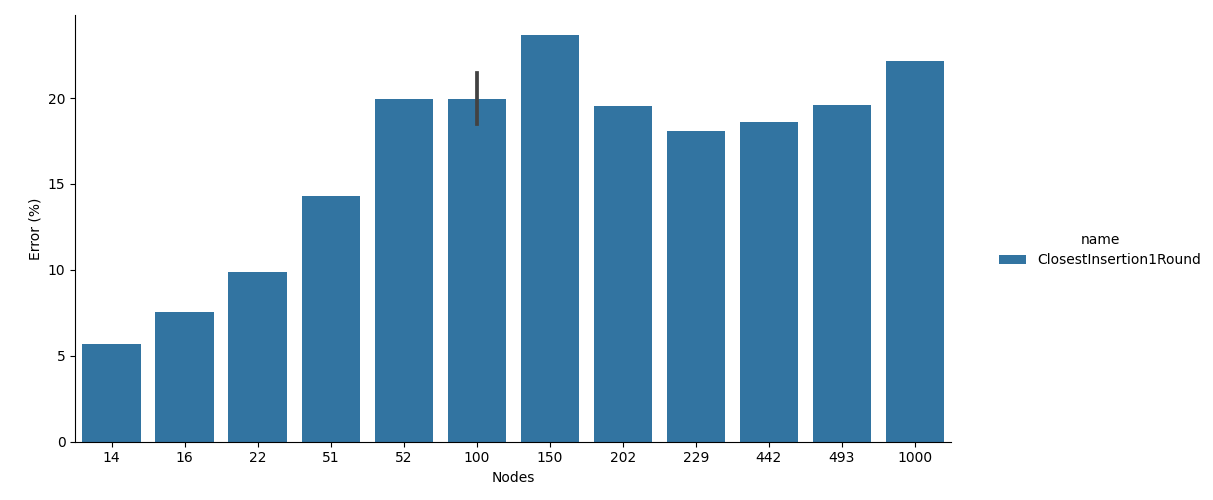
\includegraphics[width=0.9\textwidth]{./images/ClosestInsertion1Round__approximation_error_.png}

    \caption{Errore introdotto da ClosestInsertion rispetto al numero di nodi.}
    \label{fig:closest-insertion-1-round-accuracy-error}
\end{figure}


    \newpage
    \section{Analisi dei risultati}
\label{cap:performance-analysis}

\subsection{Domanda \#1}
\label{sec:question-1}

\begin{displayquote}
Eseguite i tre algoritmi che avete implementato (Held-Karp,
euristica costruttiva e 2-approssimato) sui 13 grafi del dataset.
Mostrate i risultati che avete ottenuto in una tabella come quella
sottostante. Le righe della tabella corrispondono alle istanze del
problema. Le colonne mostrano, per ogni algoritmo, il peso della
soluzione trovata, il tempo di esecuzione e l'errore relativo
calcolato come $(SoluzioneTrovata-SoluzioneOttima)/SoluzioneOttima$.
Potete aggiungere altra informazione alla tabella che ritenete
interessanti.
\end{displayquote}

\noindent Per leggibilità la tabella richiesta è stata suddivisa nelle
tabelle
\ref{table:held-karp-runtime-accuracy} (Held \& Karp),
\ref{table:mst2approx-runtime-accuracy} (MST 2-approssimato),
\ref{table:closest-insertion-runtime-accuracy} (Closest Insertion),
una per algoritmo. Abbiamo ritenuto più pratico rappresentare i tempi in millisecondi anziché secondi, visto che la maggior parte delle rilevazioni sono tempi minori al decimo di secondo.

\begin{table}[h]
    \centering

    \begin{tabular}{lrrrr}
    \toprule
    \multicolumn{5}{c}{Held \& Karp} \\
    \hline
     Istanza       &   Esatta &        Soluzione &   Tempo (ms) &   Errore (\%) \\
    \hline
    burma14.tsp   &     3323 &   3323           &          94 &        0    \\
    ulysses16.tsp &     6859 &   6859           &         393 &        0    \\
    ulysses22.tsp &     7013 &   7013           &       75295 &        0    \\
    eil51.tsp     &      426 &    986           &      126289 &      131.46 \\
    berlin52.tsp  &     7542 &  17441           &      126570 &      131.25 \\
    kroA100.tsp   &    21282 & 167464           &      128452 &      686.88 \\
    kroD100.tsp   &    21294 & 149007           &      128377 &      599.76 \\
    ch150.tsp     &     6528 &  48362           &      128392 &      640.84 \\
    gr202.tsp     &    40160 &  55127           &      128389 &       37.27 \\
    gr229.tsp     &   134602 & 176922           &      128344 &       31.44 \\
    pcb442.tsp    &    50778 & 512263           &      128303 &      908.83 \\
    d493.tsp      &    35002 & 321918           &      128277 &      819.71 \\
    dsj1000.tsp   & 18659688 &  546816520       &      128450 &     2830.47 \\
    \bottomrule
    \end{tabular}

    \caption{Tempo di esecuzione e errore introdotto da Held \& Karp rispetto alle istanze.}
    \label{table:held-karp-runtime-accuracy}
\end{table}

\begin{table}[h]
    \centering

    \begin{tabular}{lrrrr}
    \toprule
    \multicolumn{5}{c}{MST 2-approssimato} \\
    \hline
     Istanza       &   Esatta &        Soluzione &   Tempo (ms) &   Errore (\%) \\
    \hline
    burma14.tsp   &     3323 &   4258           &          34 &       28.14 \\
    ulysses16.tsp &     6859 &   7857           &          35 &       14.55 \\
    ulysses22.tsp &     7013 &   8377           &          34 &       19.45 \\
    eil51.tsp     &      426 &    563           &          35 &       32.16 \\
    berlin52.tsp  &     7542 &  10402           &          35 &       37.92 \\
    kroA100.tsp   &    21282 &  30032           &          36 &       41.11 \\
    kroD100.tsp   &    21294 &  28467           &          34 &       33.69 \\
    ch150.tsp     &     6528 &   9116           &          36 &       39.64 \\
    gr202.tsp     &    40160 &  52967           &          37 &       31.89 \\
    gr229.tsp     &   134602 & 178434           &          38 &       32.56 \\
    pcb442.tsp    &    50778 &  74254           &          41 &       46.23 \\
    d493.tsp      &    35002 &  45669           &          44 &       30.48 \\
    dsj1000.tsp   & 18659688 &  25703578   &          69 &       37.75 \\
    \bottomrule
    \end{tabular}

    \caption{Tempo di esecuzione e errore introdotto da MST 2-approssimato rispetto alle istanze.}
    \label{table:mst2approx-runtime-accuracy}
\end{table}

\begin{table}[h]
    \centering

    \begin{tabular}{lrrrr}
    \toprule
    \multicolumn{5}{c}{Closest Insertion} \\
    \hline
     Istanza       &   Esatta &        Soluzione &   Tempo (ms) &   Errore (\%) \\
    \hline
    burma14.tsp   &     3323 &   3588           &          35 &        7.97 \\
    ulysses16.tsp &     6859 &   7377           &          37 &        7.55 \\
    ulysses22.tsp &     7013 &   7703.5         &          36 &        9.85 \\
    eil51.tsp     &      426 &    487           &          36 &       14.32 \\
    berlin52.tsp  &     7542 &   9047           &          37 &       19.95 \\
    kroA100.tsp   &    21282 &  25842           &          37 &       21.43 \\
    kroD100.tsp   &    21294 &  25230           &          36 &       18.48 \\
    ch150.tsp     &     6528 &   8072           &          40 &       23.65 \\
    gr202.tsp     &    40160 &  48011           &          46 &       19.55 \\
    gr229.tsp     &   134602 & 158933           &          68 &       18.08 \\
    pcb442.tsp    &    50778 &  60235.5         &         141 &       18.63 \\
    d493.tsp      &    35002 &  41870.5         &         175 &       19.62 \\
    dsj1000.tsp   & 18659688 &   22798432       &        1110 &       22.18 \\
    \bottomrule
    \end{tabular}

    \caption{Tempo di esecuzione e errore introdotto da Closest Insertion rispetto alle istanze.}
    \label{table:closest-insertion-runtime-accuracy}
\end{table}

\noindent Una lettura più chiara dell'errore di approssimazione è invece
fornita dai grafici
\ref{fig:heldkarp-mst2approx-closestinsertion-accuracy-error-52-nodes}
 e \ref{fig:heldkarp-mst2approx-closestinsertion-accuracy-error}.
Possiamo notare come nel
secondo grafico l'errore di approssimazione di Held \& Karp (con timeout) diventi
praticamente impredicibile una volta superati i 22 nodi, tendendo comunque a crescere in media con la
dimensione del grafo.

\begin{figure}[H]
    \centering

    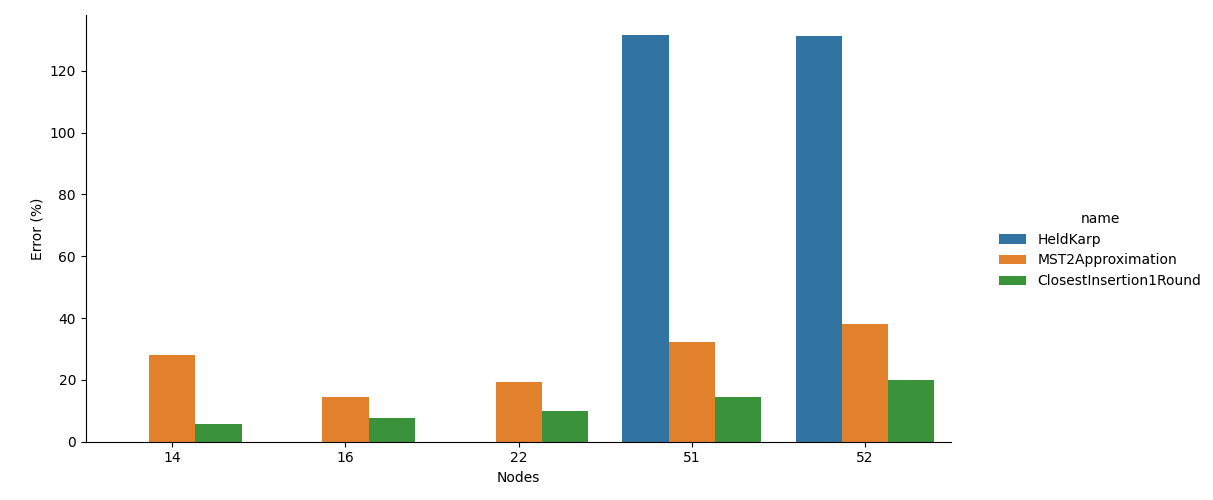
\includegraphics[width=0.9\textwidth]{./images/HeldKarp_vs_MST2Approximation_vs_ClosestInsertion1Round__approximation_error__limited_to_52_nodes_.png}

    \caption{Confronto dell'errore introdotto da Held \& Karp, MST 2-approssimato e Closest Insertion rispetto al numero di nodi (da 14 a 52)}
    \label{fig:heldkarp-mst2approx-closestinsertion-accuracy-error-52-nodes}
\end{figure}

\begin{figure}[H]
    \centering

    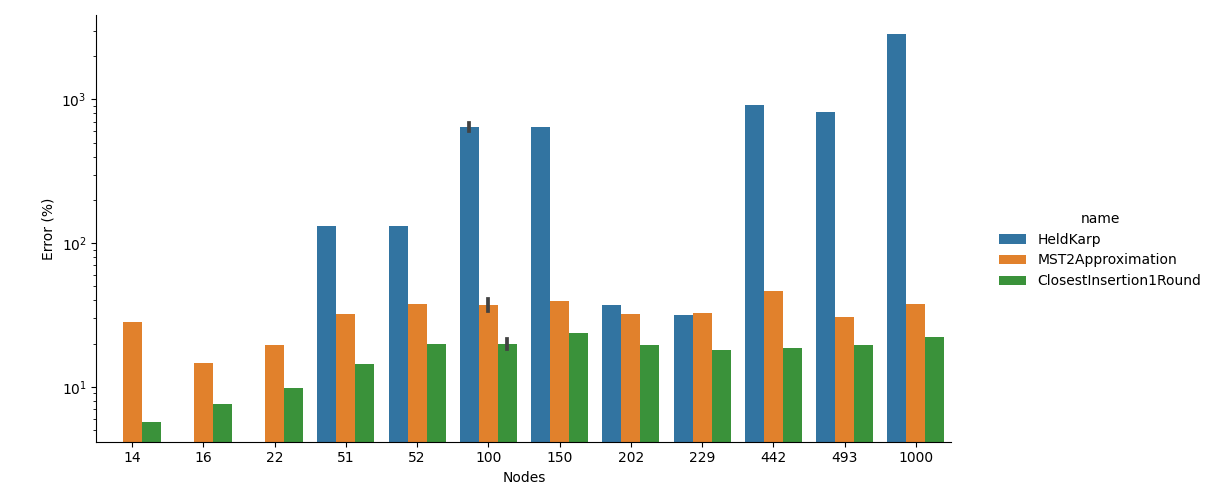
\includegraphics[width=0.9\textwidth]{./images/HeldKarp_vs_MST2Approximation_vs_ClosestInsertion1Round__approximation_error__y_log_scaled_.png}

    \caption{Confronto dell'errore introdotto da Held \& Karp, MST 2-approssimato e Closest Insertion rispetto al numero di nodi (errore in scala logaritmica)}
    \label{fig:heldkarp-mst2approx-closestinsertion-accuracy-error}
\end{figure}

\noindent Il grafico che mostra i tempi di esecuzione per tutti e tre
gli algoritmi non è stato riportato, in quanto ritenuto veramente poco
informativo: Held \& Karp va in timeout dopo i ventidue nodi (con il
timeout fissato a due minuti), mentre il meno efficiente degli altri
termina in poco più di un secondo sul grafo più grande. Abbiamo
inserito quindi il grafico
\ref{fig:mst2approx-closestinsertion-runtime} per confrontare il
runtime di MST 2-approssimato e Closest Insertion, che conferma
l'efficienza in termini di tempi di esecuzione del primo.

\begin{figure}[H]
    \centering

    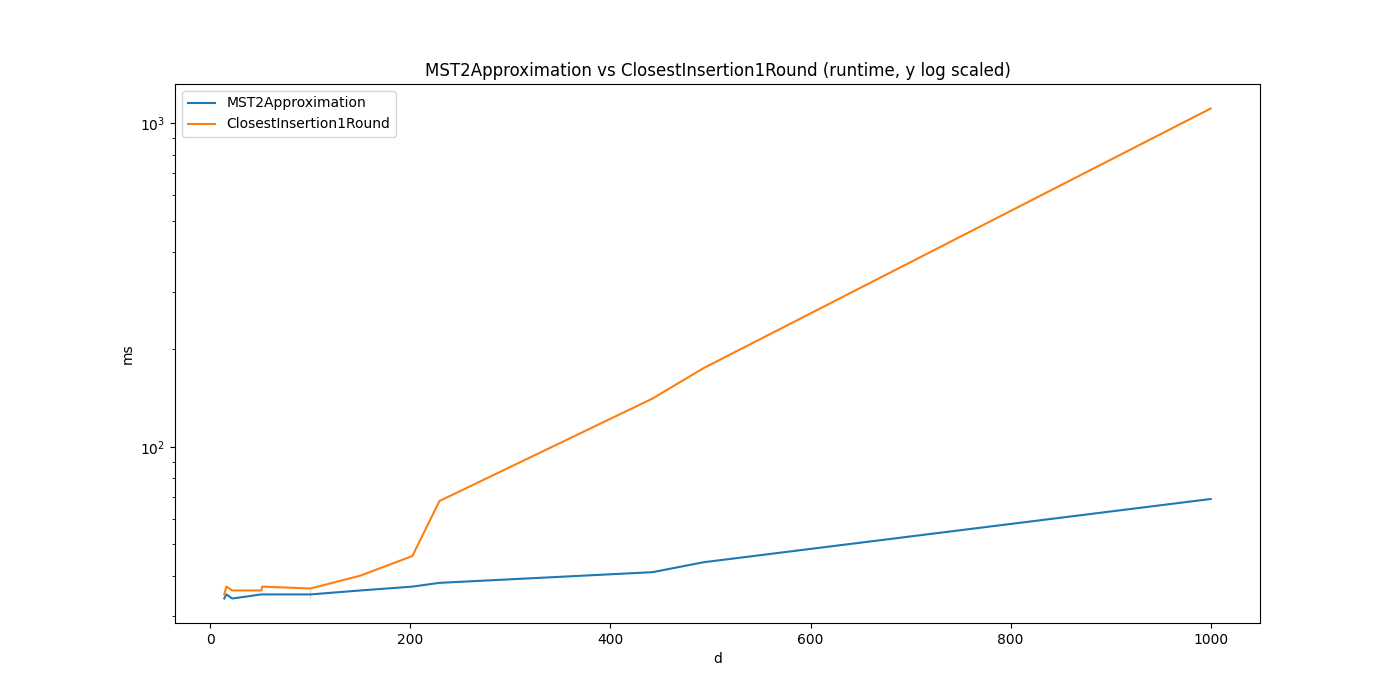
\includegraphics[width=0.9\textwidth]{./images/MST2Approximation_vs_ClosestInsertion1Round__runtime__y_log_scaled_.png}

    \caption{Confronto dei tempi di esecuzione per MST2Approximation e ClosestInsertion rispetto al numero di nodi (runtime in scala logaritmica)}
    \label{fig:mst2approx-closestinsertion-runtime}
\end{figure}

\subsection{Domanda \#2}
\label{sec:question-2}

\begin{displayquote}
Commentate i risultati che avete ottenuto: come si comportano gli
algoritmi rispetti alle varie istanze? C'è un algoritmo che riesce
sempre a fare meglio degli altri rispetto all'errore di
approssimazione? Quale dei tre algoritmi che avete implementato è
più efficiente?
\end{displayquote}

\noindent Gli algoritmi che abbiamo deciso di analizzare, come scritto
nella sezione \ref{sec:question-1}, sono Held \& Karp, MST 2-approssimato e
Closest Insertion. I dati riportati dalle tabelle e dai grafici sono di
facile lettura. Di seguito sono riportate alcune osservazioni sui
risultati ottenuti. \\

\noindent L'algoritmo che riesce
sempre a fare meglio degli altri rispetto all'errore di
approssimazione è Closest Insertion. L'algoritmo riesce a fare sempre meglio di Held Karp (con timeout) e di
MST 2-approssimato. L'errore introdotto è in media relativamente basso:
anche per input piuttosto grandi esso rimane costante intorno al 20\%
circa rispetto alla soluzione ottima. Per grafi di bassa dimensione (sotto ai 100 nodi) i tempi sono comparabili a quelli di MST 2-approssimato, per poi crescere in maniera quadratica, come ci attendevamo data la complessità temporale dell'algoritmo. \\

\noindent L'algoritmo più efficiente dal punto di vista del tempo di
esecuzione è invece MST 2-approssimato.  Quest'ultimo introduce un
errore di approssimazione non trascurabile anche su taglie piccole
dell'input, ma compensa ciò con il tempo di esecuzione dell'algoritmo
che, per dare un'idea, è inferiore ai 70 millisecondi sul grafo più
grande testato. L'approssimazione introdotta, a parte l'oscillazione
iniziale, rimane pressoché costante, intorno al 30/40\% di errore
rispetto alla soluzione ottima. Soprattutto nel caso di grafi di grossa taglia, quest'approssimazione può essere considerata soddisfacente. \\

\noindent Closest Insertion, anche se non è l'algoritmo più veloce
dei tre, ha buoni tempi di esecuzione, e nonostante sia di 2-approssimazione come l'algoritmo che usa il Minimum Spanning Tree, sembra avere un errore medio minore in pratica.

\paragraph{Osservazioni}

\begin{itemize}
    \item L'algoritmo di Held \& Karp, anche per taglie piccole dell'input
      va in timeout e sopra i 22 nodi inizia a restituire delle
      soluzioni parziali che si discostano molto dalla soluzione
      esatta. Questo fenomeno aumenta di molto soprattutto su taglie
      grosse dell'input, anche se è possibile notare un'inversione di
      tendenza per le istanze \emph{gr202} e \emph{gr229}, dove
      l'errore introdotto da Held \& Karp è simile a quello di
      MST2Approximation. È possibile ipotizzare che questo fenomeno
      si verifichi per via della distribuzione dei nodi e quindi del
      valore che gli archi assumono, ma rimane un evento limitato, tra
      l'altro a due istanze la cui sorgente di dati è la stessa. \\

    \item Nella sezione \ref{cap:extensions-and-originalities} abbiamo
      descritto altri algoritmi per la risoluzione di TSP che abbiamo
      deciso di approfondire. In particolare, abbiamo verificato
      empiricamente che l'euristica costruttiva Farthest Insertion
      funziona meglio di Closes tInsertion, e anzi, riesce a fare
      meglio per ogni istanza, con un'errore di approssimazione che
      rimane veramente basso. Per ulteriori dettagli si veda la
      sezione \ref{sec:farthest-insertion}. \\
\end{itemize}

\subsection{Altre misurazioni}

\begin{table}[h!]
    \centering

    \begin{tabular}{lrrrr}
    \toprule
    \multicolumn{5}{c}{Farthest Insertion (standard)} \\
    \hline
     Istanza       &   Esatta &        Soluzione &   Tempo (ms) &   Errore (\%) \\
    \hline
 burma14.tsp   &     3323 &   3323           &           35 &         0    \\
 ulysses16.tsp &     6859 &   6906           &           35 &         0.69 \\
 ulysses22.tsp &     7013 &   7185           &           36 &         2.45 \\
 eil51.tsp     &      426 &    452           &           36 &         6.1  \\
 berlin52.tsp  &     7542 &   8145.5         &           35 &         8    \\
 kroA100.tsp   &    21282 &  22756           &           37 &         6.93 \\
 kroD100.tsp   &    21294 &  22627           &           37 &         6.26 \\
 ch150.tsp     &     6528 &   7097.5         &           41 &         8.72 \\
 gr202.tsp     &    40160 &  43276.5         &           46 &         7.76 \\
 gr229.tsp     &   134602 & 146236           &           69 &         8.64 \\
 pcb442.tsp    &    50778 &  57289.5         &          138 &        12.82 \\
 d493.tsp      &    35002 &  38399.5         &          176 &         9.71 \\
 dsj1000.tsp   & 18659688 &   20632741 &         1114 &        10.57 \\
    \bottomrule
    \end{tabular}

    \caption{Tempo di esecuzione e errore introdotto da Farthest Insertion (standard) rispetto alle istanze.}
    \label{table:farthest-insertion-runtime-accuracy}
\end{table}

\begin{table}[h!]
    \centering

    \begin{tabular}{lrrrr}
    \toprule
    \multicolumn{5}{c}{Farthest Insertion (alternativo)} \\
    \hline
     Istanza       &   Esatta &        Soluzione &   Tempo (ms) &   Errore (\%) \\
    \hline
 burma14.tsp   &     3323 &   3323           &           35 &         0    \\
 ulysses16.tsp &     6859 &   6859           &           35 &         0    \\
 ulysses22.tsp &     7013 &   7013           &           36 &         0    \\
 eil51.tsp     &      426 &    439           &           36 &         3.05 \\
 berlin52.tsp  &     7542 &   8118           &           36 &         7.64 \\
 kroA100.tsp   &    21282 &  23373           &           36 &         9.83 \\
 kroD100.tsp   &    21294 &  22577           &           36 &         6.03 \\
 ch150.tsp     &     6528 &   6864           &           39 &         5.15 \\
 gr202.tsp     &    40160 &  45211           &           45 &        12.58 \\
 gr229.tsp     &   134602 & 148324           &           52 &        10.19 \\
 pcb442.tsp    &    50778 &  56964           &          139 &        12.18 \\
 d493.tsp      &    35002 &  39506           &          173 &        12.87 \\
 dsj1000.tsp   & 18659688 &  20599827.0 &         1110 &        10.4  \\
    \bottomrule
    \end{tabular}

    \caption{Tempo di esecuzione e errore introdotto da Farthest Insertion (alternativo) rispetto alle istanze.}
    \label{table:farthest-insertion-alt-runtime-accuracy}
\end{table}

\begin{table}[h!]
    \centering

    \begin{tabular}{lrrrr}
    \toprule
    \multicolumn{5}{c}{Simulated Annealing} \\
    \hline
     Istanza       &   Esatta &        Soluzione &   Tempo (ms) &   Errore (\%) \\
    \hline
 burma14.tsp   &     3323 &   3854         &           37 &        15.97 \\
 ulysses16.tsp &     6859 &   7580           &           37 &        10.51 \\
 ulysses22.tsp &     7013 &   7802           &           38 &        11.25 \\
 eil51.tsp     &      426 &    518           &           38 &        21.6  \\
 berlin52.tsp  &     7542 &   9412         &           41 &        24.7  \\
 kroA100.tsp   &    21282 &  29467           &           43 &        38.46 \\
 kroD100.tsp   &    21294 &  28883         &           43 &        35.64 \\
 ch150.tsp     &     6528 &   9429         &           47 &        44.43 \\
 gr202.tsp     &    40160 &  54934           &           52 &        36.79 \\
 gr229.tsp     &   134602 & 198875           &           63 &        47.75 \\
 pcb442.tsp    &    50778 &  99430           &           86 &        95.81 \\
 d493.tsp      &    35002 &  61207           &          105 &        74.87 \\
 dsj1000.tsp   & 18659688 &   100466716.0 &          293 &       438.42 \\
    \bottomrule
    \end{tabular}
    \caption{Tempo di esecuzione e errore introdotto da Simulated Annealing rispetto alle istanze.}
    \label{table:simulated-annealing-runtime-accuracy}
\end{table}

Per completezza, riportiamo nelle tabelle \ref{table:farthest-insertion-runtime-accuracy}, \ref{table:farthest-insertion-alt-runtime-accuracy} e \ref{table:simulated-annealing-runtime-accuracy} i tempi e degli errori percentuali relativi agli algoritmi presentati nella sezione \hyperref[cap:extensions-and-originalities]{Estensioni e originalità}. \\

\noindent Si osservi il curioso caso di Simulated Annealing: sembra comportarsi come un algoritmo di 2-approsimazione fino a 493 nodi, per poi esplodere nell'errore nel grafico casuale da 1000 nodi. Possiamo ipotizzare che i parametri usati in Simulated Annealing funzionino bene solo per istanze non troppo grandi. È però anche ragionevole pensare che, se \codeinline{dsj1000} non fosse un grafo costruito artificialmente, forse avremmo avuto un errore di approssimazione migliore.


    \newpage
    \section{Test}
\label{cap:tests}

Abbiamo usato i dataset di \textit{stanford-algs} per confrontare i risultati delle nostre implementazioni degli algoritmi richiesti con gli output attesi.

\noindent Abbiamo inoltre usato lo strumento di Continuous Integration \textit{Travis} per testare continuamente la solidità del codice nella nostra repository ad ogni push nel branch ``master''.

    \section{Estensioni e originalità}
\label{cap:extensions-and-originalities}

Oltre alle tre implementazioni richieste dalla consegna dell'homework,
abbiamo deciso di esplorare qualche altra estensione degli algoritmi
per il problema del commesso viaggiatore.

\subsection{TSP con Simulated Annealing}

\subsubsection{Metodo Generale}

% TODO: tagliare un po' questo paragrafo
% Simulated Annealing è un metodo di ricerca stocastico proveniente dalla Meccanica Statistica che modella lo spazio di ricerca delle soluzioni emulando il processo fisico di \textit{annealing}. L'annealing è il processo con cui un solido, portato allo stato liquido tramite riscaldamento ad alte temperature, viene portato nuovamente allo stato solido, controllando e riducendo gradualmente la temperatura. Intuitivamente, ad alte temperature gli atomi del sistema sono in uno stato altamente disordinato: l'energia del sistema è massima.
% Per riportare tali atomi in una configurazione statisticamente molto ordinata (energia minima), la temperatura del sistema deve essere gradualmente abbassata. Riduzioni di temperature troppo drastiche provocano stress termico, che rovina il sistema stesso.

\noindent Simulated Annealing è un metodo di ricerca stocastico in cui l'abilità di superare minimi locali è governata da un parametro di controllo detto "temperatura". Quando la temperatura è elevata, Simulated Annealing è simile ad una ricerca casuale di una soluzione, mentre a temperature basse, quando la temperatura è molto vicina a 0, l'algoritmo si comporta similmente a Gradient Descent e resta intrappolato nel minimo locale più vicino. \\

\noindent La temperatura è inizialmente alta, il che corrisponde ad un'alta probabilità di accettare transizioni a soluzioni non migliorative, ed è ridotta gradualmente nel tempo. La policy di raffreddamento è regolata da un altro parametro di controllo, ed emula il processo fisico di annealing, in cui un materiale solido è scaldato fino a passare allo stato liquido (dove l'energia degli atomi è massima), per essere raffreddato gradualmente per assumere una struttura cristallina (dove gli atomi tornano in uno stato di massimo ordine, e la loro energia è quindi minima). \\

\noindent Come altri metodi di ricerca stocastici, Simulated Annealing esplora l'universo di possibli soluzioni perturbando iterativamente una soluzione iniziale; a differenza di molti metodi, però, la temperatura dell'algoritmo permette di accettare anche soluzione peggiorative, il che aiuta ad evitare la convergenza in un minimo locale. \\

\noindent Ad ogni iterazione, Simulated Annealing seleziona una soluzione "vicina" alla soluzione corrente. Se la nuova soluzione ha un costo (chiamato \textit{fitness}) migliore della precedente, è sempre accettata come nuova soluzione corrente. Se invece la nuova soluzione ha un fitness peggiore, essa è accettata con una certa probabilità (legata alla distribuzione di Boltzmann). Tale probabilità è dipendente rispetto alla differenza $\Delta E$ tra le fitness delle due soluzioni confrontate e rispetto alla temperatura corrente. La probabilità di accettare soluzioni peggiorative decresce mano a mano che la temperatura diminuisce e l'ordine di grandezza di $\Delta E$ aumenta.

\noindent Abbiamo deciso di implementare Simulated Annealing perché:

\begin{itemize}
    \item Spesso converge a soluzioni sufficientemente vicine alla soluzione ottima in brevissimo tempo;
    \item È stato studiato per molti anni e la ricerca ha prodotto estensioni e miglioramenti rispetto all'algoritmo originale;
    \item Alcune varianti di Simulated Annealing sono già state applicate con successo a casi particolare di TSP, come ad esempio \textit{Compressed Annealing} per risolvere \textit{Traveling Salesman Problem with Time Windows};
    \item Se si usa Random Restart, è facile da parallelizzare;
    \item È un algoritmo citato nel corso di Intelligenza Artificiale, ma prima d'ora non avevamo mai avuto l'occasione di implementarlo e osservarlo in pratica.
\end{itemize}

\noindent I suoi punti di debolezza, invece, sono:

\begin{itemize}
    \item È non deterministico ed è difficile prevedere quanto la soluzione ritornata possa essere peggiore della soluzione ottima;
    \item Se la temperatura iniziale non è inizializzata correttamente rispetto all'input atteso, le performance dell'algoritmo degradano e le soluzioni ritornate possono essere molto distanti da quella ottima.
    \item Se la temperatura viene raffreddata troppo velocemente, le performance degradano similmente al punto precedente.
    \item Se le dimensioni degli input dell'algoritmo differiscono molto e i parametri di Simulated Annealing sono fissati, è difficile ottenere buoni risultati su tutte le istanze di input.
\end{itemize}

\subsubsection{Scelta della soluzione iniziale}

Simulated Annealing richiede una soluzione di partenza, la quale sarà poi iterativamente sottoposta a perturbazioni per esplorare soluzioni vicine. Nel nostro caso, abbiamo deciso di usare l'euristica \textbf{Nearest Neighbors}. Le regioni per questa scelta sono:

\begin{itemize}
    \item È molto veloce e la soluzione ritornata non è troppo distante dalla soluzione ottima di TSP;
    \item È una tra le euristiche costruttive proposte nell'homework che non abbiamo implementato come metodo a sé, ed eravamo curiosi di implementarla.
\end{itemize}

Per essere ragionevolmente sicuri di partire da una buona soluzione iniziale, Nearest Neighbors è lanciato 10 volte. Di queste 16 esecuzioni, la soluzione selezionata è il circuito Hamiltoniano ritornato di peso minore.

\subsubsection{Scelta delle soluzioni vicine}

Il criterio di selezione di Simulated Annealing è strettamente dipendente al problema a cui è applicato. Nel caso di TSP, abbiamo deciso di generare perturbazioni in 3 modi diversi, scelti casualmente ad ogni iterazione.

\textbf{TODO}: presentare brevemente questi 3 modi

\subsubsection{Scelta della temperatura iniziale}

Inizialmente avevamo fissato la temperatura inizale a $1.000.000$. Questa scelta sembrava funzionare per la maggiorparte dei dataset dell'homework, ma le performance degradavano di molto per grafi con più di 150 nodi. \\

% TODO: aggiungere link a https://www.researchgate.net/publication/227061666_Computing_the_Initial_Temperature_of_Simulated_Annealing

\noindent Abbiamo quindi adottato il metodo di inizializzazione di Ben-Ameur, che si basa sul coefficiente di accettazione iniziale $\chi{}_0$. $\chi{}_0$ rappresenta la percentuale di transizioni sfavorevoli di simulated annealing che ci aspettiamo vengano accettate alla prima iterazione dell'algoritmo. Solitamente il valore di $\chi{}_0$ è compreso nell'intervallo $[0.8, 0.\overline{99}]$. Nel nostro caso, $\chi{}_0 = 0.94$ ci ha dato i risultati medi migliori su tutti i dataset. \\

\noindent Per come abbiamo inizializzato i parametri del metodo di Ben-Ameur, grafi di dimensione più alta partiranno da una temperatura più alta, il che equivale ampliare il raggio di ricerca delle soluzioni all'aumentare della complessità dell'input.

\subsubsection{Reheating}

Una delle estensioni di Simulated Annealing prevede di riscaldare nuovamente la temperatura dopo un certo numero di iterazioni. L'intuizione è che questo dà la possibilità di ampliare lo spazio di ricerca delle soluzioni, e riduce maggiormente le possibilità che l'algoritmo converga in un minimo locale. \\

\noindent Nel nostro caso, la temperatura è aumentata ad intervalli regolari di valori via via decrescenti all'aumentare delle iterazioni di Simulated Annealing. La formula di reheating è la seguente, dove $\tau{}$ è la temperatura corrente, $\tau{}_0$ è la temperatura iniziale, $i$ è l'iterazione corrente, $\rho$ è il fattore di reheating:

\begin{equation}
    \tau{} = \frac{\tau{}_0 \cdot \rho{}}{10 \cdot (i + 1)}
\end{equation}

L'ampiezza degli intervalli di \textit{reheating} è fissata e data dalla seguente formula, dove $\tau{}_0$ rappresenta la temperatura iniziale:

\begin{equation}
    max\{ \frac{\tau{}_0}{4000}, 100 \}
\end{equation}

\noindent Tali formule sono state scelte in modo sperimentale, poiché non abbiamo trovato riferimenti a riguardo nella letteratura.

\subsubsection{Parallelismo}

Uno dei punti di forza di Simulated Annealing è che, se si applica Random Restart, l'algoritmo è banalmente parallelizzabile.
Random Restart consiste nel lanciare un algoritmo di ricerca stocastico (nel nostro caso, Simulated Annealing) un certo numero di volte, restituendo solamente la migliore soluzione trovata. \\

\noindent Abbiamo definito la classe di utilità \codeinline{parallel\_executor} in \codeinline{SimulatedAnnealing/parallel.h}, la quale si occupa di eseguire una funzione \textit{higher-order} su un certo numero di thread paralleli e di selezionare la migliore soluzione ottenuta. Essa è stata utilizzata per eseguire in parallelo molteplici istanze indipendenti di Simulated Annealing. In particolare, il numero di istanze eseguite in parallelo è par al numero di core fisici della CPU del computer di esecuzione.

\subsubsection{Steady Steps}

\noindent Per evitare il rischio di abbassare la temperatura del sistema troppo velocemente, e per esplorare un maggior numero di possibili soluzioni, l'algoritmo genera un numero costante di soluzioni vicine rispetto alla soluzione corrente prima di effettuare un passo di annealing (che consiste nel moltiplicare la temperatura corrente per il coefficiente di raffreddamento $\beta$). \\

\noindent Abbiamo determinato sperimentalmente che un buon numero di \textit{steady steps} è 5.

\subsubsection{Criterio di convergenza}

\noindent Nella letteratura sono presenti diversi criteri per determinare quando Simulated Annealing ha effettuato un numero sufficiente di iterazione. Per cercare di garantire una certa robustezza alla nostra implementazione, ne abbiamo applicati diversi:

\begin{itemize}
    \item \textbf{Massimo numero di iterazioni}: è il criterio più semplice, consiste nel fermarsi una volta superato un certo numero predefinito di \textit{annealing steps};
    \item \textbf{Raggiungimento temperatura minima}: l'algoritmo si ferma la temperatura ha raggiunto un valore prossimo a 0. Noi consideriamo $1 \cdot 10^{-16}$ come temperatura minima;
    \item \textbf{Miglior soluzione ripetuta}: la ricerca si ferma se la miglior soluzione individuata non cambia per un certo numero di iterazioni consecutive. Noi consideriamo fino a $150$ ripetizioni consecutive della stessa migliore soluzione prima di dichiarare la convergenza.
\end{itemize}

\noindent Tutte le condizioni elencate sopra sono "in OR", ovvero l'algoritmo termina non appena si verifica almeno una delle condizioni di convergenza.

\subsection{Closest Insertion}
\label{sec:closest-insertion}

\emph{Closest Insertion} è una delle euristiche impiegabili per la
risoluzione problema del TSP in modo approssimato. Questa euristica
è molto simile a \emph{Farthest Insertion} (si veda \ref{sec:farthest-insertion}),
infatti differisce da essa solo per la selezione del vertice $k$
da inserire nel circuito parziale $C$.

In particolare, in questo caso viene scelto il vertice $k$ non presente
nel circuito $C$ che minimizza $\delta (k, C) = \min_{h \in C} w(h, k)$.
Sostanzialmente viene scelto il vertice $k$ più vicino al ciclo $C$,
ma che non è ancora incluso in esso.

\subsubsection{Implementazione}

Il codice è sostanzialmente simile a quello riportato nel listato
\ref{listing:farthest-insertion}, con la differenza che per
\emph{Closest Insertion} si effettua la scelta del nuovo nodo
con \mintinline{c++}{utils::select_new_k} passandogli come quarto
argomento un comparatore che permette, in questo caso, di
minimizzare $\delta (k, C)$.

\begin{listing}[!ht]
\begin{minted}{c++}
// the comparator will be passed to std::max_element.
const auto min_comparator = [](const auto& x, const auto& y) {
    return x.second > y.second;
};
\end{minted}
\caption{Differenza di implementazione per Closest Insertion rispetto a Farthest Insertion.}
\label{listing:closest-insertion-diff}
\end{listing}

\subsubsection{Approssimazione}

Questa euristica permette di trovare una soluzione $\log(n)$-approssimata,
ma è possibile dimostrare che il fattore di approssimazione può essere
ulteriormente abbassato fino ad avere una soluzione $2$-approssimata.

I risultati che abbiamo ottenuto con closest insertion sono illustrati
dalla tabella \ref{table:closest-insertion-runtime-accuracy} e dal grafico
\ref{fig:closest-insertion-accuracy-error}.

\begin{figure}[H]
    \centering

    \begin{tabular}{lrrrr}
    \toprule
    \multicolumn{5}{c}{Closest Insertion} \\
    \hline
    Instance & Exact & Solution &   Time (ms) &   Error (\%) \\
    \hline
    burma14.tsp   &     3323 &       3664 &          35 &       10.26 \\
    ulysses16.tsp &     6859 &       7054 &          36 &        2.84 \\
    ulysses22.tsp &     7013 &       7499 &          36 &        6.93 \\
    eil51.tsp     &      426 &        480 &          37 &       12.68 \\
    berlin52.tsp  &     7542 &       8626 &          35 &       14.37 \\
    kroA100.tsp   &    21282 &      24661 &          38 &       15.88 \\
    kroD100.tsp   &    21294 &      22998 &          38 &        8    \\
    ch150.tsp     &     6528 &       7763 &          40 &       18.92 \\
    gr202.tsp     &    40160 &      45660 &          46 &       13.7  \\
    gr229.tsp     &   134602 &     163597 &          52 &       21.54 \\
    pcb442.tsp    &    50778 &      58297 &         142 &       14.81 \\
    d493.tsp      &    35002 &      40537 &         180 &       15.81 \\
    dsj1000.tsp   & 18659688 &   22510610 &        1127 &       20.64 \\
    \bottomrule
    \end{tabular}

    \caption{ClosestInsertion runtime and accuracy error}
    \label{table:closest-insertion-runtime-accuracy}
\end{figure}

\begin{figure}[H]
    \centering

    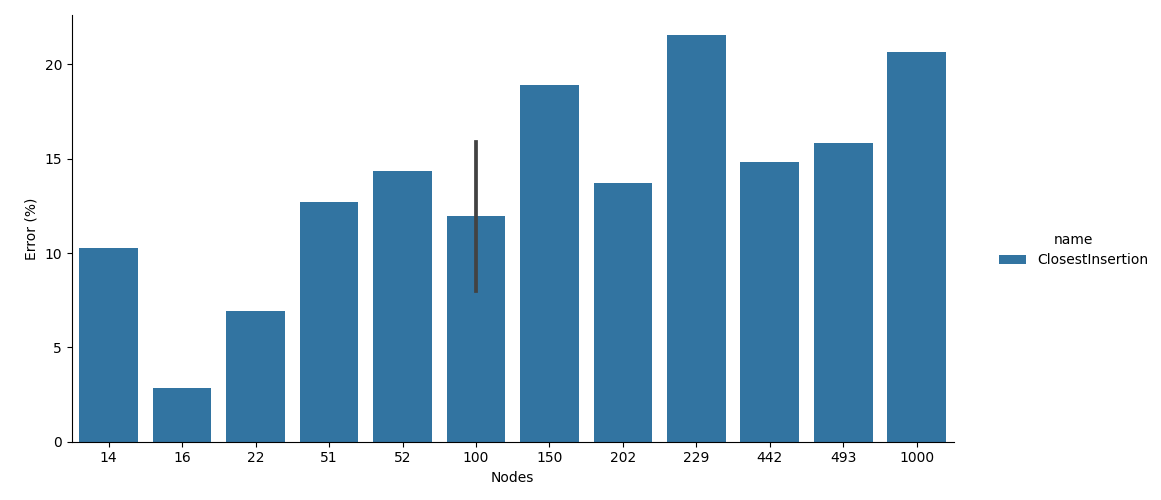
\includegraphics[width=0.9\textwidth]{./images/ClosestInsertion__approximation_error_.png}

    \caption{ClosestInsertion accuracy error scaling by nodes}
    \label{fig:closest-insertion-accuracy-error}
\end{figure}

\subsubsection{Osservazioni}

Data la netta dualità con FarthestInsertion, è doveroso analizzare
le differenze tra i due algoritmi. Dalla tabella 
\ref{table:closest-farthest-insertion-runtime-accuracy} 
e dal grafico \ref{fig:closest-farthest-insertion-accuracy-error}
è possibile notare che per quanto riguarda il runtime i due algoritmi
sono perfettamente alla pari, infatti minimizzare o massimizzare la
funzione $\delta (k, C)$ dal punto di vista del tempo di esecuzione
non comporta differenze. Dal punto di vista dell'errore di 
approssimazione invece FarthestInsertion riesce a fare mediamente
meglio di ClosestInsertion. Da sottolineare anche il fatto che 
FarthestInsertion riesce ad eliminare completamente l'errore di
approssimazione su istanze molto piccole.

\begin{figure}[H]
    \centering

    \begin{tabular}{lrrrrrr}
    \toprule
    \multicolumn{1}{c}{ } & \multicolumn{3}{c}{Closest Insertion} & \multicolumn{3}{c}{Farthest Insertion} \\
    \hline
    Instance & Solution &   Time (ms) &   Error (\%) & Solution &   Time (ms) &   Error (\%) \\
    \hline
    burma14.tsp   &     3664 &          35 &       10.26 &       3323 &          35 &        0    \\
    ulysses16.tsp &     7054 &          36 &        2.84 &       6859 &          35 &        0    \\
    ulysses22.tsp &     7499 &          36 &        6.93 &       7013 &          35 &        0    \\
    eil51.tsp     &      480 &          37 &       12.68 &        439 &          36 &        3.05 \\
    berlin52.tsp  &     8626 &          35 &       14.37 &       8118 &          36 &        7.64 \\
    kroA100.tsp   &    24661 &          38 &       15.88 &      23373 &          36 &        9.83 \\
    kroD100.tsp   &    22998 &          38 &        8    &      22577 &          36 &        6.03 \\
    ch150.tsp     &     7763 &          40 &       18.92 &       6864 &          41 &        5.15 \\
    gr202.tsp     &    45660 &          46 &       13.7  &      45211 &          46 &       12.58 \\
    gr229.tsp     &   163597 &          52 &       21.54 &     148324 &          52 &       10.19 \\
    pcb442.tsp    &    58297 &         142 &       14.81 &      56964 &         140 &       12.18 \\
    d493.tsp      &    40537 &         180 &       15.81 &      39506 &         176 &       12.87 \\
    dsj1000.tsp   & 22510610 &        1127 &       20.64 &   20599827 &        1125 &       10.4  \\
    \bottomrule
    \end{tabular}

    \caption{ClosestInsertion vs FarthestInsertion runtime and accuracy error}
    \label{table:closest-farthest-insertion-runtime-accuracy}
\end{figure}

\begin{figure}[H]
    \centering

    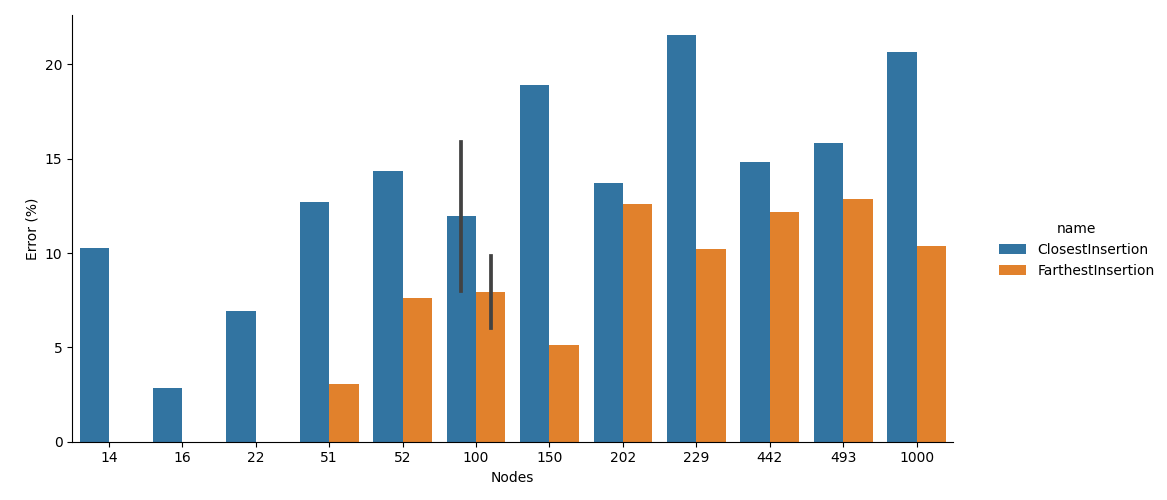
\includegraphics[width=0.9\textwidth]{./images/ClosestInsertion_vs_FarthestInsertion__approximation_error_.png}

    \caption{ClosestInsertion vs FarthestInsertion accuracy error scaling by nodes}
    \label{fig:closest-farthest-insertion-accuracy-error}
\end{figure}

    \newpage
    \section{Conclusioni}
\label{cap:conclusions}

In questa relazione abbiamo descritto gli algoritmi e relative le
scelte di implementazione, tempi di esecuzione, l'errore di
approssimazione e ottimizzazioni utilizzate per rendere i programmi
più efficienti. \\

\noindent Nella sezione \ref{cap:performance-analysis} abbiamo
risposto alle 2 principali domande dell'homework, mentre nella sezione
\ref{cap:benchmark-process} abbiamo descritto il processo di benchmark
adottato, pensato per essere quanto più affidabile e stabile
possibile.  Nelle sezioni \ref{cap:code-structure},
\ref{cap:implementation-choices} e \ref{cap:algorithms} abbiamo invece
discusso i dettagli tecnici, quali struttura, scelte implementative e
codice degli algoritmi. \\

\noindent La sezione \ref{cap:extensions-and-originalities} descrive
infine le estensioni esplorate per soddisfare la nostra curiosità e
arricchire il nostro bagaglio accademico, e permettendoci di esplorare
alternative anche migliori. \\

\noindent Questo progetto ci ha permesso di sperimentare diversi
algoritmi di approssimazione ed euristiche per un problema non banale
il cui algoritmo deterministico ha complessità non
polinomiale. L'impossibilità di calcolare una soluzione esatta anche
per dimesioni medio/grandi dell'input ci ha spinto a cercare algoritmi
nuovi e migliori rispetto ai tre scelti inizialmente per
l'homework. Abbiamo infatti sperimentato nuove euristiche come
FarthestInsertion e la sua implementazione alternativa
FarthestInsertionAlternative; abbiamo implementato SimulatedAnnealing,
che risolve il problema in un modo completamente diverso e escogitato
un modo di ottenere approssimazione ancora migliori semplicemente
sfruttando gli stessi algoritmi eseguiti con inizializzazione
differente.\\

\noindent Il progetto è disponibile anche come repository pubblica su Github:

\begin{center}
\href{https://github.com/jkomyno/algorithms-hw2}{github.com/jkomyno/algorithms-hw2}
\end{center}



    % TODO: appendix with results read from CSV
    \newpage
    \appendix
\section{Tabelle tempi di esecuzione}
\label{cap:runtime-tables}


  \end{document}
